\title{Monografia - LUARKIAN}

\documentclass[
	% -- opções da classe memoir --
	12pt,				% tamanho da fonte
    oneside,			% Tipo de impressão, frente-verso(twoside) ou apenas frente(oneside)
	a4paper,			% tamanho do papel. 
	% -- opções da classe abntex2 --
	chapter=TITLE,		% títulos de capítulos convertidos em letras maiúsculas
	% -- opções do pacote babel --    
	english,			% idioma adicional para hifenização
	brazil				% o último idioma é o principal do documento    
	]{abntex2}
    
    %\renewcommand{\ABNTEXpartfontsize}{\normalsize}
	%\renewcommand{\ABNTEXchapterfontsize}{ \large}
	%\renewcommand{\ABNTEXsectionfontsize}{\normalsize}
	%\renewcommand{\ABNTEXsubsectionfontsize}{\normalsize}

% ---
% Pacotes básicos 
% ---
\usepackage{lmodern}			% Usa a fonte Latin Modern			
\usepackage[T1]{fontenc}		% Selecao de codigos de fonte.
\usepackage[utf8]{inputenc}		% Codificacao do documento (conversão automática dos acentos)
\usepackage{lastpage}			% Usado pela Ficha catalográfica
\usepackage{indentfirst}		% Indenta o primeiro parágrafo de cada seção.
\usepackage{color}				% Controle das cores
\usepackage{graphicx}			% Inclusão de gráficos
\usepackage{microtype} 			% para melhorias de justificação
\usepackage{todonotes}
\usepackage{tabularx}
\usepackage{amssymb}


\definecolor{algColor}{RGB}{255,206,206} % rgb(255, 206, 206)

% Pacotes para algoritmos/pseudo-código
\usepackage{listings}

\renewcommand{\lstlistingname}{Programa}

\lstset
{ %Formatting for code in appendix
    language=C,
    basicstyle=\footnotesize,
    numbers=left,
    stepnumber=1,
    frame = single,
    showstringspaces=false,
    tabsize=2,
    breaklines=true,
    xleftmargin=10pt,
    breakatwhitespace=false,
    extendedchars=true,
    literate={á}{{\'a}}1 
             {ã}{{\~a}}1
             {é}{{\'e}}1
             {í}{{\'i}}1
             {õ}{{\~o}}1
             {ç}{{\c{c}}}1,
}

\usepackage{xcolor}
\colorlet{punct}{red!60!black}
\definecolor{background}{HTML}{EEEEEE}
\definecolor{delim}{RGB}{20,105,176}
\colorlet{numb}{magenta!60!black}

\lstdefinelanguage{json}{
    basicstyle=\normalfont\ttfamily,
    numbers=left,
    numberstyle=\scriptsize,
    stepnumber=1,
    numbersep=8pt,
    showstringspaces=false,
    breaklines=true,
    frame=lines,
    backgroundcolor=\color{background},
    literate=
     *{0}{{{\color{numb}0}}}{1}
      {1}{{{\color{numb}1}}}{1}
      {2}{{{\color{numb}2}}}{1}
      {3}{{{\color{numb}3}}}{1}
      {4}{{{\color{numb}4}}}{1}
      {5}{{{\color{numb}5}}}{1}
      {6}{{{\color{numb}6}}}{1}
      {7}{{{\color{numb}7}}}{1}
      {8}{{{\color{numb}8}}}{1}
      {9}{{{\color{numb}9}}}{1}
      {:}{{{\color{punct}{:}}}}{1}
      {,}{{{\color{punct}{,}}}}{1}
      {\{}{{{\color{delim}{\{}}}}{1}
      {\}}{{{\color{delim}{\}}}}}{1}
      {[}{{{\color{delim}{[}}}}{1}
      {]}{{{\color{delim}{]}}}}{1},
}


\renewcommand{\lstlistlistingname}{Lista de códigos}

% Configura a ``Lista de Códigos'' conforme as regras da ABNT (para abnTeX2)
\begingroup\makeatletter
\let\newcounter\@gobble\let\setcounter\@gobbletwo
  \globaldefs\@ne \let\c@loldepth\@ne
  \newlistof{listings}{lol}{\lstlistlistingname}
  \newlistentry{lstlisting}{lol}{0}
\endgroup

\renewcommand{\cftlstlistingaftersnum}{\hfill--\hfill}

\let\oldlstlistoflistings\lstlistoflistings
\renewcommand{\lstlistoflistings}{%
   \begingroup%
   \let\oldnumberline\numberline%
   \renewcommand{\numberline}{\lstlistingname\space\oldnumberline}%
   \oldlstlistoflistings%
   \endgroup}
% ---
% Pacotes adicionais, usados apenas no âmbito do Modelo Canônico do abnteX2
% ---
\usepackage{lipsum}				% para geração de dummy text
% ---


% ---
% Pacotes de citações
% ---
%\usepackage[brazilian,hyperpageref]{backref}	 % Paginas com as citações na bibl
\usepackage[alf, abnt-etal-cite=2]{abntex2cite}	% Citações padrão ABNT

% --- 
% CONFIGURAÇÕES DE PACOTES
% --- 

\usepackage{abntex_ufrr_dcc}


% PACOTES DE ALGORITMO

\usepackage{algpseudocode,algorithm}
% Declaracoes em Português

\algrenewcommand\algorithmicend{\textbf{FIM}}
\algrenewcommand\algorithmicdo{\textbf{FAÇA}}
\algrenewcommand\algorithmicwhile{\textbf{ENQUANTO}}
\algrenewcommand\algorithmicfor{\textbf{PARA}}
\algrenewcommand\algorithmicforall{\textbf{PARA TODO}}
\algrenewcommand\algorithmicif{\textbf{SE}}
\algrenewcommand\algorithmicthen{\textbf{ENTÃO}}
\algrenewcommand\algorithmicelse{\textbf{SENÃO}}
\algrenewcommand\algorithmicreturn{\textbf{RETORNE}}
\algrenewcommand\algorithmicfunction{\textbf{FUNÇÃO}}
% New definitions
\algnewcommand\algorithmicswitch{\textbf{ESCOLHA}}
\algnewcommand\algorithmiccase{\textbf{CASO}}
\algnewcommand\algorithmicassert{\texttt{assert}}
\algnewcommand\Assert[1]{\State \algorithmicassert(#1)}%
% New "environments"
\algdef{SE}[SWITCH]{Switch}{EndSwitch}[1]{\algorithmicswitch\ #1\ \algorithmicdo}{\algorithmicend\ \algorithmicswitch}%
\algdef{SE}[CASE]{Case}{EndCase}[1]{\algorithmiccase\ #1}{\algorithmicend\ \algorithmiccase}%
\algtext*{EndSwitch}%
\algtext*{EndCase}%


% Rearranja os finais de cada estrutura
\algrenewtext{EndWhile}{\algorithmicend\ \algorithmicwhile}
\algrenewtext{EndFor}{\algorithmicend\ \algorithmicfor}
\algrenewtext{EndIf}{\algorithmicend\ \algorithmicif}
\algrenewtext{EndFunction}{\algorithmicend\ \algorithmicfunction}

% O comando For, a seguir, retorna 'para #1 -- #2 até #3 faça'
\algnewcommand\algorithmicto{\textbf{até}}
\algrenewtext{For}[3]%
{\algorithmicfor\ #1 $\gets$ #2 \algorithmicto\ #3 \algorithmicdo}


% ---
% Configurações do pacote backref
% Usado sem a opção hyperpageref de backref
%\renewcommand{\backrefpagesname}{Citado na(s) página(s):~}
% Texto padrão antes do número das páginas
%\renewcommand{\backref}{}
% Define os textos da citação
%\renewcommand*{\backrefalt}[4]{
%	\ifcase #1 %
%		Nenhuma citação no texto.%
%	\or
%		Citado na página #2.%
%	\else
%		Citado #1 vezes nas páginas #2.%
%	\fi}%
% ---

% ---
% Informações de dados para CAPA e FOLHA DE ROSTO
% ---
\titulo{INEXT: Um Sistema Computacional para Localização Indoor de Objeto com RFID}

\autor{LUARKIAN KAYPE DE SOUSA}
\local{Boa Vista - RR}
\data{2019}
\orientador{Dr. Herbert Oliveira Rocha}

\tipotrabalho{Monografia}

\preambulo{Monografia de Graduação apresentada ao Departamento de Ciência da Computação da Universidade Federal de Roraima como requisito para a obtenção do grau de Bacharel em Ciência da Computação.}

%Trabalho de conclusão de curso  na área de Verificação de Software desenvolvido na UFRR com o %objetivo \textcolor{red}{VERIFICAR O PADRÃO DOS OUTROS TCC} de gerar casos de teste para %sistemas embarcados críticos	

% ---

%-- Informações de dado para a FOLHA DE APROVAÇÃO
\renewcommand{\dataDefesa}{10 de Julho de 2019}
\renewcommand{\orientadorBanca}{Prof. Dr. Herbert Oliveira Rocha}
\renewcommand{\primeiroMembroBanca}{Prof. MSc. Acauan Cardoso Ribeiro}
\renewcommand{\segundoMembroBanca}{Prof. Dr. Leandro Nelinho Balico}

% ---
% Configurações de aparência do PDF final

% alterando o aspecto da cor azul
\definecolor{blue}{RGB}{41,5,195}

% informações do PDF
\makeatletter
\hypersetup{
     	%pagebackref=true,
		pdftitle={\@title}, 
		pdfauthor={\@author},
    	pdfsubject={\imprimirpreambulo},
	    pdfcreator={LaTeX with abnTeX2},
		pdfkeywords={abnt}{latex}{abntex}{abntex2}{trabalho acadêmico}, 
		colorlinks=true,       		% false: boxed links; true: colored links
    	linkcolor=blue,          	% color of internal links
    	citecolor=blue,        		% color of links to bibliography
    	filecolor=magenta,      	% color of file links
		urlcolor=blue,
		bookmarksdepth=4
}
\makeatother
% --- 

% --- 
% Espaçamentos entre linhas e parágrafos 
% --- 

% O tamanho do parágrafo é dado por:
\setlength{\parindent}{1.3cm}

% Controle do espaçamento entre um parágrafo e outro:
\setlength{\parskip}{0.2cm}  % tente também \onelineskip

% ---
% compila o indice
% ---
\makeindex
% ---

% ----
% Início do documento
% ----
\begin{document}

% Retira espaço extra obsoleto entre as frases.
\frenchspacing 

% ----------------------------------------------------------
% ELEMENTOS PRÉ-TEXTUAIS
% ----------------------------------------------------------
% \pretextual

% ---
% Capa
% ---
\imprimircapa
% ---

% ---
% Folha de rosto
% (o * indica que haverá a ficha bibliográfica)
% ---
\imprimirfolhaderosto
% ---

% ---
% Inserir folha de aprovação
% ---
\imprimirfolhadeaprovacao
% ---
% Dedicatória
% ---
\begin{dedicatoria}
   \vspace*{\fill}
   \centering
   \noindent
   \textit{Dedico com muito amor àquela que luta todos os dias pela minha educação, chora as minhas lágrimas, sorri com as minhas alegrias. Minha mãe Maria Francisca.} \vspace*{\fill}
\end{dedicatoria}
% ---

% ---
% Agradecimentos
% ---
\begin{agradecimentos}[Agradecimentos]
\par
Primeiramente, agradeço a minha família, por sempre estar ao meu lado nos momentos mais difíceis da faculdade, pelos conselhos e pelo incentivo em todos estes anos de faculdade.
\par
Agradeço ao meu orientador, professor Herbert Oliveira, por todo apoio e por todas as orientações no desenvolvimento deste projeto, além dos incentivos para vida pós faculdade.

\par
Agradeço aos professores do DCC que durantes estes anos de curso foram fonte de aprendizado e incentivos durante aulas e que cada uma pode contribuir de alguma forma no meu desenvolvimento como aluno e futuro profissional.

\end{agradecimentos}
% ---

% ---
% Epígrafe
% ---
\begin{epigrafe}
    \vspace*{\fill}
	\begin{flushright}
		\textit{''Uma flecha só pode ser lançada se for puxada para trás. Então, quando a vida te puxar para trás, significa que ela vai te lançar para algo grande. Apenas mantenha o foco e continue mirando.''  - Autor Desconhecido }
	\end{flushright}
\end{epigrafe}
% ---

% ---
% RESUMOS
% ---

% resumo em português
\setlength{\absparsep}{18pt} % ajusta o espaçamento dos parágrafos do resumo
\begin{resumo}[Resumo]
A ampla utilização da Internet das Coisas (IoT) tem estimulado uma crescente demanda por
sistema de localização em ambiente fechados, tendo em vista que o sistema de posicionamento global (GPS)
pode não ser eficiente ou mesmo não funcionar tão bem em tal ambiente. A tecnologia de identificação por radiofrequência (RFID) facilita a construção
de sistemas com baixo custo para localização e identificação de objetos. Neste trabalho propomos um sistema computacional
que utiliza leitores e etiquetas RFID passivas, para o gerenciamento e controle de ativos, sendo capaz de localizar e
identificar objetos etiquetados em edifícios.

 \vspace{\onelineskip}
 
 \noindent 
 \textbf{Palavras-chaves:} Localização Indoor, RFID, IoT.
\end{resumo}

%\begin{resumo}[Abstract]
% \begin{otherlanguage*}{english}
%  The proliferation and adoption of the Internet of Things (IoT) has stimulated the growing to localization system indoors since the global positioning system (GPS) does not work so well in such an environment. RFID technology makes it easy to build low-cost systems for locating and identifying objects. In this work we propose a tool that uses passive RFID readers and tags for asset management and control being able to locate and identify tagged objects in buildings.
%
%   \vspace{\onelineskip}
% 
%   \noindent 
%   \textbf{Key-words}: location of objects, identification of objects, RFID, passive RFID tag.
% \end{otherlanguage*}
%\end{resumo}
% ---
% inserir lista de ilustrações
% ---
\pdfbookmark[0]{\listfigurename}{lof}
\renewcommand{\listfigurename}{Lista de Figuras}
\listoffigures*
\cleardoublepage
% ---

% ---
% inserir lista de tabelas
% ---
\pdfbookmark[0]{\listtablename}{lot}
\renewcommand{\listtablename}{Lista de Tabelas}
\listoftables*
\cleardoublepage
% ---

% ---
% inserir lista de abreviaturas e siglas
% ---
%\begin{siglas}
%  \item[GPS] Global Positioning System
%  \item[IoT]  Internet of Things
%  \item[RFID] Radio Frequency Identification
%  \item[RSS] Received Signal Strength
%  \item[RSSI] Received Signal Strength Indication
%  \item[RTLS] Real Time Location System
%  \item[UML]  Unified Modeling Language
%  \item[WLAN] Wireless Local Area Network
%  \item[WSN]  Wireless Sensor Network
%  \item[AOA]  Angle of Arrival
%  \item[TDOA] Time Difference of Arrival

%\end{siglas}
% ---

% ---
% inserir lista de símbolos
% ---
% \begin{simbolos}  
%   \item[$ \Gamma $] \todo{Atualizar esta lista!} Letra grega Gama
%   \item[$ \Lambda $] Lambda
%   \item[$ \zeta $] Letra grega minúscula zeta
%   \item[$ \in $] Pertence
% \end{simbolos}
% % ---

% ---
% inserir o sumario
% ---
\pdfbookmark[0]{\contentsname}{toc}
\renewcommand{\contentsname}{Sumário}
\tableofcontents*
\cleardoublepage
% ---



% ----------------------------------------------------------
% ELEMENTOS TEXTUAIS
% ----------------------------------------------------------
\textual
% ----------------------------------------------------------
% Introdução
% ----------------------------------------------------------
\chapter{INTRODUÇÃO}

%===========================================================
%INTRODUÇÃO
%===========================================================
A localização é um tipo de informação situacional muito importante, no contexto geral temos aplicações que fornecem a 
localização de algo, por exemplo para casas nós temos ruas, número da casa, e bairro. No sistema de posicionamento global 
para um ponto temos latitude e longitude. Entretanto quando se restringe o ambiente considerando apenas edifícios e o 
alvo para itens de uso geral (cadeiras, mesas, notebooks, desktop, etc) seja para realizar monitoramento, acompanhamento do 
fluxo e/ou rastreamento poucas ferramentas proporcionam isso com baixo custo \cite{rfid2009review}.


As conexões entre computadores que chamavam de 
redes de computadores quando se referia a um conjunto de computadores autônomos interconectados \cite{tenenbaum2002}, 
esse conceito está absoleto pois não se tem apenas computadores conectados, mas diversos dispositivos que podem ser ou 
não semelhantes, podendo ser cameras, sensores, \textit{smartphones}, ou qualquer objeto que possua um 
hardware com capacidade de conectividade \cite{iot2016SBRC}.


Com os avanços tecnológios interações com objetos tornou-se cada vez mais frequênte, isso se deu a um paradigma 
que visa uma interligação de objetos em rede para interação e cooperação podendo mudar ou não a forma como as atividades 
rotineiras serão realizadas, esse modelo é chamado de \textit{Internet of Things (IoT)} \cite{realtimeRFID2016}.


A IoT que também está relacionada com computação ubíqua é chamada de tecnologia do futuro, a comunicação de diferentes dispositivos, 
edificios ou qualquer equipamente que possua um microcontrolador ou microprocessador embutido e que podem se conectar a 
redes para assim ter uma comunicação com outros se encaixa nessa relação 
\cite{mechanismRFID2006}.


No trabalho de \citeonline{IotMartins} é realizado uma abordagem para \textit{smart cities}, que são 
aplicações que visam a troca de inormações entre veículos, \textit{smartphones}, semáforos e qualquer 
outro dispositivo capaz de enviar e receber dados, com a troca de dados entre os dispositivos pretende-se 
ter um melhor fluxo de carros em uma cidade, gerenciamento de desperdicios e monitoramento de qualidade de vida na cidade. 


\citeonline{landmarc} apresenta um sistema de localização RFID, que foi aplicado para facilitar a gestão de 
hospitais e outras organizações, para melhorar os seviços, economizar custos e reduzirem os riscos. O sistema também era 
utilizado para monitorar pacientes infcciosos e garantir resposta no tempo adequado para emergências.


A interligação dos objetos as redes possibilitou que o meio científico propursessem várias maneiras de localização em ambientes 
confinados, visto que o GPS não funciona tão bem para a solução proposta, tendo em vista que um edifício possui 
muitas salas ou/e andares, e com o GPS não seria possível saber em qual sala por não ter uma planta baixa do prédio ou 
informar qual o andar o objeto se encontra pois o GPS retornaria para a aplicação as coordenadas de latitude e longitude \cite{rfid2009review}.


Para solucionar essa incapacidade de localização do GPS, inúmeas aplicações foram propostas para a localização indoor. 
Aplicações que utilizam tecnologia infravermelho difuso para estimar a posição, sistemas que utilizam adaptadores de rede 
padrão IEEE 802.11 para rastrear os objetos no interior do prédio, sistemas baseados na tecnologia ultra-sônica e 
tambem sistemas que utilizam RFID para rastreio indoor foram propostos \cite{mechanismRFID2006}. 


O RFID foi a tecnologia escolhida por proporcinar a utilização de etiquetas que não necessitam de uma fonte de alimentação 
para seu funcionamento, pois são alimentadas pelas ondas eletromagnéticas emitidas pela antena do leitor, sendo que isso não 
é possivel em outras tecnologias. Uma outra funcionalidade do RFID é a possibilidade de identificação das etiquetas que possui 
uma ID única.


% %===========================================================
% %MOTIVAÇÃO
% %===========================================================

%===========================================================
%DEFINIÇÃO DO PROBLEMA
%===========================================================
\section{Definição do Problema}
A dificuldade de localizar objetos em ambientes confinados ou fechados, cria uma necessidade de novas ferramentas para 
tal aplicação sendo que o GPS não se aplica a tal problema por na localização do GPS os prédios são apresentados como um edifício sem salas e divisórias, sem contar o custo beneficio para anexar módulos de GPS aos objetos, isso iria deixar o protótipo caro. Contudo, o motivo desta pesquisa é auxiliar na localização de objetos permanentes (como computadores e moveis) 
em ambientes de uma forma que não tenha o custo elevado quanto a utiliação do 
GPS\cite{mechanismRFID2006}.

\par
\begin{comment}
Os edifícios e construções dificultam o envio de sinais de rádio emitidos pelos satélites e dispositivos que fazem uso do GPS, 
por essa questão sua utilização torna-se inviável para aplicações que consistem em localizar objetos em ambientes fechados, 
além que o tempo-de-luz transitório fica difícil e caro para fazer sua medição \cite{rfid2009review}.
\end{comment}

%dependendo da forma que os dados são armazedados e recuperados possibilita a identificação automatica utilizando tags e leitores, 

Localizar e identificar objetos em certos ambientes têm grande importância quando se quer gerenciar e controlar ativos, 
por exemplo em comércios, indústrias ou instituições de ensino que possuem uma gama de bens que podem ser movimentados dentro do local, 
poder identificar o objeto que está sendo movido e saber em que local o objeto está, é de grande importância para ter um maior 
controle sobre os bens \cite{realtimeRFID2016}. 

A tecnologia RFID é um meio de comunicação sem fio que utiliza compo eletromagnéticos de 
radiofrequencia para identificar etiquetas. As etiquetas podem ser passivas, ativas e 
semi-passivas. As etiquetas semi-ativa e ativas possuem uma fonte de alimentação, a semi-ativa só emite sinais 
quando entra em contato com o leitor, já ativa emite os sinais a todo momento, as etiquetas passivas não 
possuem fonte de alimentação entrando em funcionanmento apenas quando as ondas eletromagnéticas emitidas pelo 
leitor os alimentam\cite{realtimeRFID2016}. As funcionalidade da tecnoliga RFID fez com que muitas técnicas de localização fossem propostas.

\begin{comment}
\par
Muitas técnicas de localização baseadas em RFID foram propostas, sendo com foco em objetos móveis ou estacionários, contudo algumas dessas 
técnicas fazem uso de etiquetas ativas a fim de obter melhores estimativas,
\end{comment}


O problema considerado neste trabalho é expresso na seguinte questão: 
\textbf{Como projetar um sistema computacional capaz de localizar e identificar objetos em tempo real com baixo custo, em ambientes confinados ou fechados, garantindo confiabilidade na informações fornecidade e auxiliando usuários no gerenciamento de bens por meio da utilização de radio frequência?}

%===========================================================
%OBJETIVOS GERAIS E ESPECIFICOS
%===========================================================
\section{Objetivos}
O objetivo principal deste trabalho é projetar e desenvolver um sistema computacional autonomo para o gerenciamento de objetos com RFID 
em ambientes confinados ou fechados, utilizando técnicas de localização e identificação de redes IoT.


Objetivos específicos:
\begin{enumerate}

    \item Analisar soluções computacionais de baixo custo que são capazes de localizar objetos indoor;
    
    \item Identificar algoritmos para localização de objetos indoor;
        %, verificando se podem ser adaptados no prótotipo a ser desenvolvido;
%    \item Localizar objetos em ambientes confinados utilizando tags RFID.
    
%    \item Identificar objetos em ambientes internos utilizando tags RFID.
    
%    \item Monitorar objetos caso mudem de localização no ambiente, a fim de ter um controle sobre os objetos cadastrados no sistema.
    
    \item Projetar e desenvolver um prótotipo de um sistema capaz de localizar e identificar objetos em tempo real, no âmbito confinado utilizando RFID; e
    
    \item Validar o método proposto com o próposito de examinar sua eficácia e aplicabilidade.
\end{enumerate}


\begin{comment}
%===========================================================
%METODOLOGIA PROPOSTA
%===========================================================
\section{Metodologia Proposta}

%===========================================================
%CONTRIBUIÇÕES PROPOSTAS
%===========================================================
\section{Contribuições propostas}
As contribuições propostas deste trabalho são:
\begin{enumerate}
    \item A implementação de um sistema para localização de objetos. O Metódo utilizado visa localizar objeto sem alta precisão, porém é viável para controle de acervos.
    \item O sistema desevolvido pode auxiliar no controle e ainda facilitar o levantamento de todos os bens do proprietário.
\end{enumerate}

\end{comment}


%===========================================================
%ORGANIZAÇÃO DO TRABALHO
%===========================================================
\section{Organização do trabalho}
A introdução deste trabalho apresentou: o contexto, definição do problema, objetivos, metodologia e contribuições 
dessa pesquisa. Os capítulos restantes são organizados da seguinte forma:

No \autoref{chapter:conceitos}, \textbf{Conceitos e Definições}, são apresentados fundamentos teóricos que abordam os 
seguintes assuntos: sistemas embarcados, sistemas de comunicação e localização, algoritmos utilizados em localização, e modelagem.

\par
No \autoref{chapter:correlatos}, \textbf{Trabalhos Correlatos}, são apresentados trabalhos correlatos a utilização de RFID e localização.

\par
No \autoref{chapter:metodo}, \textbf{Método Proposto}, é descrito as etapas da solução proposta neste trabalho, de 
forma a mostrar a arquitetura do sistema proposto e componentes necessários para a aplicação.

\par
No \autoref{chapter:cronograma}, \textbf{Cronograma}, é descrito as próximas fases do desenvolvimento deste trabalho.

%No \autoref{chapter:resultados} \textbf{Resultados Experimentais}, descreve-se a execução de uma avaliação experimental 
\par
E por fim no \autoref{chapter:consideracoes}, \textbf{Considerações Parciais e Trabalhos Futuros}, será apresentado as 
considerações parciais e próximos passo deste trabalho.


% ----------------------------------------------------------
% Conceitos e Definições
% ----------------------------------------------------------
\chapter{CONCEITOS E DEFINIÇÕES}
\begin{comment}
\label{chapter:conceitos}
Este capítulo tem como objetivo apresentar os principais conceitos e definições abordados neste trabalho, tais como: Linguagens de descrição de hardware, Verificação de sistemas e Técnicas de Compiladores.

%============================
%Linguagens de descrição de hardware
%============================



\section{Linguagens de descrição de hardware}

As linguagens de descrição de hardware(HDL) foram desenvolvidas com o intuito de auxiliar a criação de circuitos lógicos com grande número de elementos e com uma gama de abstrações lógicas e eletrônicas \cite{thomas2008verilog}. \textcolor{red}{Entre os exemplos, podemos citar: \textit{VDHL}, \textit{Verilog} e \textit{SystemC}.}

\par
Segundo \cite{christen1999vhdl}, linguagens de descrição de hardware são linguagens de programação utilizadas com o intuito de descrever o comportamento de um determinado circuito e processos, técnica conhecida como modelagem. Os modelos descritos em HDL são utilizados como entrada para um simulador, onde o mesmo pode ter seu comportamento analisado.

\begin{figure}[htb]
	\begin{center}
    \caption{\label{fig:waveform_fig}Waveform de multiplexador de duas entradas}
	\includegraphics[scale=0.55]{Figuras/Waveform_multiplex.png}
	\end{center}
    \legend{Fonte: Própria}
\end{figure}

\par
As HDL's trazem consigo diversas vantagens, entre elas códigos independentes de tecnologia e fabricante, podendo ser portatéis e reutilizáveis\cite{cappelattipraticando}. As lingugens mais modernas, tais como VHDL e \textit{Verilog}, possuem suporte tanto a descrição do circuito propriamente dito quanto ao comportamento que o mesmo deve exercer\cite{christen1999vhdl}.

\par
\textcolor{red}{O \textit{Verilog}, como já citado, é uma linguagem de descrição de \textit{hardware} que fornece diversos níveis de abstração para desenvolvimento de sistemas digitais\cite{thomas2008verilog}. A linguagem foi desenvolvida para ser simples e efetiva nos diversos níveis de abstração incluindo o suporte ao desenvolvimento, verificação, síntese e testes de \textit{software}.\cite{IEEEVerilogLanguage}.}

\par
\textcolor{red}{O VHDL é uma linguagem de descrição de hardware amplamente utilizada concebida na década de 80, visto uma necessidade do Departamento de defesa dos Estados Unidos da América\cite{cappelattipraticando}. Assim como o Verilog, suporta desenvolvimento, verificação, síntese, e testes de \textit{hardware}\cite{IEEEVHDLLanguage}.}

\par
\textcolor{red}{Ambas as linguagens apesentam similaridades, sendo a linguagem VHDL escolhida para este projeto devido a linguagem apresentar maior gama de recursos tanto para o desenvolvimento quanto para oa auxilio nos testes.}\todo{O motivos da escolha ainda esta fraco, devido a familiaridades entre ambas as linguagens, ainda não sobre como colocar o motivo da escolha.}

%============================
%VHDL
%============================
\subsection{VHSIC Hardware Description Language - VHDL}\todo{Revisar textos e verificar a necessidade de mais exemplo}

VHDL é uma linguagem de descrição de hardware destina a ser utilizada em todas as etapas da criação de sistemas eletrônicos, sendo, desenvolvimento, verificação, síntese e teste de circuitos\cite{IEEEVHDLLanguage}.

\par
\textcolor{red}{Segundo \cite{cappelattipraticando}, o VHDL apresenta três principais pilares: Abstração, que consiste na descrição com diferentes níveis de detalhes; modularidade, que permite a divisão do projeto em vários blocos ou módulos para posterior interconexão; e hierarquia, permitindo que módulos ser compostos por submódulos e estes ter níveis de abstração diferentes, dependendo da necessidade do projeto. Devido a esta versatilidade que a linguagem VHDL foi selecionada para o projeto.}

\par
\textcolor{red}{Segundo \cite{IEEEVHDLLanguage}, é necessário um padrão para formatação da descrição em VHDL: \textit{Entity} (Pinos de entada/saída) e \textit{Architecture} (Arquitetura). A \textit{Entity} ou entidade representa o bloco onde são declaradas as entradas e as saídas do circuito utilizadas em todo o sistema, conforme apresentado na \autoref{fig:biblioteca_entidade}. A \textit{Architecture} ou arquitetura, apresentado na \autoref{fig:arquitetura}, define a relação entre entrada e saídas declaradas na entidade, podendo tais especificações serem completas ou parciais. Assim como em outras linguagens bibliotecas podem ser adicionadas, para que novos tipo possam ser utilizados no projeto.} 

\begin{figure}[thp]
\caption{\label{fig:biblioteca_entidade} Exemplo de declaração de bibliotecas e entidade.}
	\begin{center}
    \begin{minipage}{0.6\textwidth}
    \begin{lstlisting}       
library ieee;
use IEEE.STD_LOGIC_1164.ALL

ENTITY full_adder IS PORT(
	x1,x2,cin: in std_logic;
   S,count:out std_logic);
END full_adder;
\end{lstlisting}
    \end{minipage}
	\end{center}
    \legend{Fonte: Própria.}
\end{figure}

\begin{figure}[thp]
\caption{\label{fig:arquitetura} Exemplo de declaração da arquitetura no VHDL.}
	\begin{center}
    \begin{minipage}{0.6\textwidth}
    \begin{lstlisting}       
ARCHITECTURE behavioral OF full_adder IS
BEGIN
	s<=x1 XOR x2 XOR cin;
    cout<=(x1 AND x2) OR (x1 AND cin) OR (b AND cin);
END behavioral;

\end{lstlisting}
    \end{minipage}
	\end{center}
    \legend{Fonte: Própria.}
\end{figure}

\par
\textcolor{red}{Segundo \cite{cappelattipraticando},} uma descrição em VHDL pode conter diferentes níveis de abstração:
\begin{itemize}
  \item \textbf{Comportamental:} Permite descrever o circuito através de laços e processos. O circuito é definido em forma de um algoritmo, utilizando construção similares as utilizadas em linguagem de programação.
  
  \item \textbf{Transferencia de registradores:} Englobando a representação do dispositivo em nível de trasnferencia entre registradores, que consiste a utilização de funções lógicas combinacionais e registradores.
  
  \item \textbf{Estrutural:} O circuito é descrito mais próximo da implementação real, podendo ser definidas portas lógicas com atrasos unitarios ou com atrasos detalhados.
\end{itemize}

\todo[inline]{Tabala de caracteristicas do vhdl}

%============================
%PORTAS LÓGICAS
%============================
\subsection{Portas lógicas}

Segundo \citeauthor{idoeta1982elementos} conceito de portas lógicas é baseado na conhecida álgebra de Boole ou álgebra booleana, desenvolvida pelo matemático inglês George Boole em 1854. A álgebra booleana é representada por apenas dois valores, sendo eles o $0$ e $1$ e através disso expressar a relação entre entrada e saída dentro de um circuito. As portas lógicas podem ser construídas a partir de diodos, transmissões e resistores interconectados de modo que a saída seja o resultante de uma operação lógica básica realizada sobre as entradas \cite{tocci2003sistemas}. A figura \autoref{fig:algebra_booleana} apresenta um exemplo de álgebra booleana sem a utilização de diagramas.

\begin{figure}[htb]
	\begin{center}
    \caption{\label{fig:algebra_booleana}Exemplo de algebra booleana, onde A=0, B=1, C=1 e D=1.}
	\includegraphics[scale=0.70]{Figuras/algebra_booleana.png}
	\end{center}
    \legend{Fonte: \cite{tocci2003sistemas}}
\end{figure}

\par
Ainda segundo \citeauthor{tocci2003sistemas}, devido a esta característica, a álgebra booleana possui três operações básicas, \texttt{OR} (ou), \texttt{AND} (e) e \texttt{NOT} (não). Tal conjunto de operações também é denominado de operações booleanas e via utilização de tabela-verdade é possível descrever as saídas baseando-se nas entradas e na operação aplicada. Cada operação booleana possui sua tabela verdade(\autoref{fig:exemplo_diagrama}), mas também sua representação em forma de diagrama.

\begin{figure}[htb]
	\begin{center}
    \caption{\label{fig:exemplo_diagrama}Simbolo e tabela verdade para uma porta OR de três entradas.}
	\includegraphics[scale=0.60]{Figuras/exemplo_diagrama.png}
	\end{center}
    \legend{Fonte: \cite{tocci2003sistemas}}
\end{figure}

\begin{figure}[htb]
	\begin{center}
    \caption{\label{fig:exemplo_circuito} Representação de circuito lógico, utilizando portas lógicas.}
	\includegraphics[scale=0.60]{Figuras/exemplo_circuito.png}
	\end{center}
    \legend{Fonte: \cite{tocci2003sistemas}}
\end{figure}

A \autoref{fig:exemplo_circuito} apresenta um circuito lógico formado pelas portas básicas da álgebra booleana. O circuito apresenta 3 entradas representadas pelas letras A, B e C, mas também formada por duas portas \textit{AND}, uma porta \textit{NOT} e uma porta \textit{OR}. Cada uma destas portas representando operações a serem realizadas, podendo receber como entrada um valor inicial ou resultante de outra porta, como no exemplo ocorre com a última porta \textit{AND}.

%============================
%VERIFICAÇÃO DE SISTEMAS
%============================
\section{Verificação de sistemas}
\textcolor{red}{ contexto inicial da verificação de sistemas, faz-se necessário o entendimento e a diferenciação entre verificação e validação. Verificação e validação possuem o intuíto de mostrar que determinado \textit{software} funcione conforme o especificado, além de satisfazer as especificações do cliente\cite{sommerville2011engenharia}.} 

\par
Segundo \cite{sargent2005verification}, Verificação é o processo de determinar se um modelo computacional obtido por discretização de um modelo matemático de um evento físico e o código que implementa o modelo computacional pode ser usado para representar o modelo matemático do evento com precisão suficiente e validação é o processo de determinar se um modelo matemático de um evento físico representa o evento físico real com precisão suficiente.

\par
\textcolor{red}{A verificação consite identificação de erros e provavéis problemas que um componente pronto possa apresentar, enquanto a validação busca analisar se tal componete esta seguindo os requisitos pré-definidos para sua construção\cite{koscianski2007qualidade}. O teste de programa, na qual o software  é executado com dados de teste é a principal forma de validação, porém, tecnicas de verificação, tais como, inspeção e revisões também podem integrar a etapa de validação\cite{sommerville2011engenharia}.}

\subsection{Diagrama de decisão binária}
Diagrama de decisão binária é um grafo aciclico para representação de funcões boolenas. Existe uma ordem total rigorosa na ocorrência de variáveis à medida que uma atravessa o grafo da raiz para a folha. Dado o exemplo,\autoref{fig:bdd_fig}, \textit{f=(a$\lor$b)$\land$(c$\lor$d)} e utilizando a ordenação de variavél a < b < c < d. Dada a atribuição de valores booleanos as variaveis a, b, c e d, pode-se decidir se a atribuição torna a fórmula verdadeira atravessando o início do gráfico na raiz e ramificação em cada nó. Definindo a,c e d = 1 e c = 0 leva a folha de rótulo 1, portanto, a fórmula é verdadeira para essa tarefa\cite{clarke1994model}.

\begin{figure}[htb]
	\begin{center}
    \caption{\label{fig:bdd_fig}Arvore de decisão binária}
	\includegraphics[scale=0.20]{Figuras/Arvore_BDD.png}
	\end{center}
    \legend{Fonte: \cite{clarke1994model}}
\end{figure}

%============================
%BOUNDED MODEL CHECKING
%============================
\subsection{\textit{Bounded Model Checking}}
Segundo, \citeauthor{rocha2015verificaccao}, \textit{Bounded Model Checking} (BMC) é um tipo especial de \textit{Model Checking} que geralmente utiliza o método de satisfabilidade booleana, o qual tem sido introduzido como uma técnica complementar para diagrama de decisão binaria para aliviar o problema da explosão de estados, visto que a técnica de \textit{Model Checking} busca todos os estados possíveis para verificação.

\par
Segundo \cite{rocha2015verificaccao} o \textit{Bounded Model Checking} é a verificação de uma propriedade especifica em uma determinada profundidade: dado um sistema de transições M, uma propriedade $\phi$, e um limite (\textit{bound}) $k$, o BMC desenrola o sistema $k$ vezes e traduz o sistema em uma condição de verificação(CV) $\psi$ tal que $\psi$ é satisfeito se e somente se $\phi$ tem um contra-exemplo de profundidade menor ou igual a $k$.

\par
O \textit{Extended SMT-Based Bounded Model Checker} (ESBMC) é um \textit{Bounded Model Checking} baseado em satisfabilidade booleana (SAT) que permite verificação aritmética de overflow e undeflow, segurança de ponteiros, limite de array, de gerar propriedades de segurança em programas em C/C$++$. ESBMC utiliza uma versão modificada do CBMC no \textit{front-end} para analisar o código ANSI-C e para gerar as condições de verificação através de execução simbólica \cite{cordeiro2012smt,rocha2015verificaccao}.

\par
No ESBMC, o programa analisado é modelado em um sistema de transição de estados, conforme a trupla: M=(S,R,$S_{0}$), o qual é gerado um grafo de controle de fluxo(GFC), onde S representa o conjunto de estados, R $\subseteq$ SxS representa as transições e S $\subseteq$ S representa o conjuto de estados iniciais. Um estado s $\in$ S consiste no valor do contador de programa(PC) e os valores de todas as variáveis dos programas. O estado inicial $S_{0}$ atribui o inicio do programa GFC ao PC, desta forma o ESBMC identifica as transições, conforme a formula lógica, $\gamma$=($S_{i}$,$S_{i+1}$) que captura as retrições sobre os valores correspondntes do PC e das variáveis do programa\cite{cordeiro2012smt}.

\par
Segundo o site da ferramenta, a ferramenta permite ao usuário indicar propriedades adicionais usando assertivas que também são verificadas. O ESBMC converte as condições usando diferentes técnicas de background para posteriormente passar para verificador SMT. Outra vantagem é a ferramenta permitir verificação de software single-thread e multi-thread.

%============================
%REDES DE PETRI
%============================
\subsection{Redes de petri}
Redes de petri são ferramentas de modelagem gráfica/matemática. Como ferramenta gráfica são utilizadas como comunicação visual, como fluxogramas, por exemplo e como ferramenta matemática podem configurar modelos matemáticos que regem o comportamento dos sistemas. A grade premissa desta ferramenta é descrever sistemas de processamento de informações caracterizados como concorrentes, assíncronos, distribuídos, paralelos, não deterministas e/ou estocásticos\cite{murata1989petri}.

\par
\textcolor{red}{ As redes de petri são compostas, conforme apresentado na \autoref{fig:rede_petri}, grafos direcionais compostos por nós e arcos. Os nós representam as transições e eventos e os arcos representam os pesos. Dentro desta representação, os arcos e eventos são componentes passivos enquanto as transições são ativos. A principal vantagem da utilização das redes de petri esta relacionado ao chamado "\textit{Token game}" que consiste no comportamento da rede de petri, em outras palavras, representa o funcionamento do sistema representado pela rede\cite{halder2006}.}

\begin{figure}[htb]
	\begin{center}
    \caption{\label{fig:rede_petri}Rede de petri}
	\includegraphics[scale=0.40]{Figuras/rede_petri.png}
	\end{center}
    \legend{Fonte: \cite{halder2006}}
\end{figure}
%============================
%VERIFICAÇÃO DE HARDWARE
%============================
\subsection{Verificação formal de hardware}

A verificação de hardware, por meio da simulação, via assegurar que uma implemetação, descrição do hardware em qualquer qualquer nível de abstração da hierarquia e hardware, atinja suas especificações, propriedades que devem ser respeitadas para que a corretude do mesmo seja comprovada \cite{gupta1992formal}. A Verificação formal de hardware consiste na utilização dos conceitos de verificação formal, mas também técnicas para corretude de circuitos lógicos, ou seja, consiste na utilização de modelos matemáticos para descrição de propriedade e/ou de comportamento de um dado sistema.\cite{kropf2013introduction}.

\par
\textcolor{red}{Entre as abordagens utilizadas verificação formal de hardware consiste em tanto a implementação quanto a especificação estarem descritas em lógica formal, neste caso a corretude será obtida através da comprovada relação entre a implementação e a especificação\cite{seger1992introduction}. A especificação formal consiste na descrição do comportamento, bem como, das propriedades do sistema em linguagem matemática, tornando-se crucial para o processo de verificação. Na implementação formal, o nível de abstração, tais como, \textit{Gate level} e RTL são importantes informações para o desenvolvimento do formalismo, bem como as classes, por exemplo se o circuito é sequencial ou combinacional, se utiliza pipeline, etc.\cite{kropf2013introduction}.}

\par
\textcolor{red}{A utilização de \textit{Model Checking} também se faz presente nos modelos formais de verificação de hardware, onde apenas é utilizado o comportamento dos circuitos na verificação, de modo a verificar a se as propriedades  presentes são satisfeitas. Para isso, são utilizados os conceitos da lógica proposicional, que por meio da utilização de fórmulas que representem as propriedades dos estados, é possível realizar as verificações necessárias\cite{seger1992introduction}.}
 
%============================
%VERIFICAÇÃO DE SOFTWARE
%============================
\subsection{Verificação formal de software}

Segundo \citeauthor{rocha2015verificaccao}, o uso de software tem sido feito em muitas áreas, tais como, infraestruturas industriais de missão critica e de segurança.  Logo, existe a necessidade de garantir a corretude destes sistemas. Devido a isso, a verificação formal tem sido utilizada em três principais abordagens, sendo elas~\cite{cousot2010gentle,d2008survey}:
\begin{itemize}
 \item \textcolor{red}{\textbf{Métodos dedutivos:} Produzem provas matemáticas formais de corretude usando provadores de teoremas ou assistentes de prova para execução da prova e necessitam da interação humana para prover os argumentos\cite{cousot2010gentle};}
  \item \textbf{Verificação de modelos:} Exploram exaustivamente modelos de execuções de programa, que podem ser sujeitos a explosão combinatória, necessário a intervenção humana para geração dos modelos.\cite{rocha2015verificaccao};
  \item \textcolor{red}{\textbf{Analise estática:} Engloba diversas técnicas para calcular automaticamente informações sobre o comportamento de um programa sem executá-lo, sendo utilizado em otimização de código e verificação em compiladres\cite{d2008survey}.}
\end{itemize}

Ainda segundo \citeauthor{rocha2015verificaccao}, na verificação formal apresentam-se dificuldades, tais como: quais as propriedades são de interesse na verificação no tempo de execução; e impossibilidade matemática de provar a corretude de propriedades não triviais no comportamento de programas, devido ao computador ser um dispositivo finito\cite{cousot2010gentle}. 

\todo[inline]{Sugiro adicionar um exemplo de verificacao de SW.}

%============================
%LÓGICA PROPOSICIONAL
%============================
\subsection{Lógica proposicional}
A lógica proposicional é uma linguagem formal onde é definida um alfabeto e conectivos proposicionais, e um conjunto de regras gramaticais, as quais serão utilizadas para construção das proposições\cite{souza2017logica}. Porém apesar de importante, ela é limitada, não podendo expressar sentenças elementares importantes, tais como a da aritmética elementar. Por exemplo:
\begin{enumerate}
\item Todos são mortais.
\item Alguém é bondoso.
\end{enumerate}
Na lógica preposicional, não poderiam ser analisadas, pois não teria como decompor ambas em sentença e assim não teria como analisar as diferenças entre ambas\cite{abe2002introducao}. Contudo, no exemplo:
\begin{enumerate}
\item Existem cavalos com patas verdes.
\end{enumerate}
A relação criada pela frase poderia  a ser analisada pela lógica proposicional\cite{abe2002introducao}.

Segundo \citeauthor{souza2017logica}, alfabeto da lógica proposicional é formado por símbolo de pontuação, símbolos proposicionais e conectivos proposicionais, onde cada um apresenta uma função em específico, sendo:
\begin{itemize}
\item \textbf{Símbolos de pontuação: }Apenas dois símbolos de pontuação são utilizados o "(" e o ")".
\item \textbf{Símbolos proposicionais:} São utilizados para representar as proposições, onde um símbolo \textit{P} pode ser utilizado para representar uma proposição qualquer, por exemplo: \textit{P}="Está chovendo". O conjunto de símbolos proposicionais é infinito e enumerável, sendo possível representar infinitos e enumerável conjunto de proposições.
\item \textbf{Conectivos proposicionais:} São os símbolos usando frequentemente na matemática. Os símbolos recebem a seguinte denominação: 
\begin{enumerate}
\item \textbf{$\neg$}: Representa a partícula de negação, ou seja, "Não".
\item \textbf{$\lor$}: Representa a partícula "Ou"
\item \textbf{$\land$}: Representa a partícula "E"
\item \textbf{$\rightarrow$}: Representa a partícula "Se então ou implica".
\item \textbf{$\Leftrightarrow$}: Representa a partícula "Se, e somente se".
\end{enumerate} 
\end{itemize}

Ainda segundo \citeauthor{souza2017logica}, existem as fórmulas que são constituídas de forma indutiva, a partir de símbolos do alfabeto conforme as regras apresentadas abaixo:
\begin{itemize}
\item Todo o símbolo preposicional é uma fórmula
\item Se \textit{H} é uma fórmula, então ($\neg$\textit{H}), a negação de \textit{H}, é uma fórmula.
\item Se \textit{H} e \textit{G} são fórmulas, então a disjunção de \textit{H} e \textit{G}, dada por (\textit{H} $\lor$ \textit{G}), é uma fórmula.
\item Se \textit{H} e \textit{G} são fórmulas, então a conjunção de \textit{H} e \textit{G}, dada por (\textit{H} $\land$ \textit{G}), é uma fórmula.
\item Se \textit{H} e \textit{G} são fórmulas, então a implicação de \textit{H} e \textit{G}, dada por (\textit{H} $\rightarrow$ \textit{G}), é uma fórmula. Neste caso, \textit{H} é o antecedente e \textit{G} consequente da fórmula.
\item Se \textit{H} e \textit{G} são fórmulas, então a bi-implicação de \textit{H} e \textit{G}, dada por (\textit{H} $\leftrightarrow$ \textit{G}), é uma fórmula. Neste caso, \textit{H} é o lado esquerdo e \textit{G} o lado direito da fórmula.
\end{itemize}


%============================
%Property Specification Language - PSL
%============================
\subsection{Linguagem de especificação de propriedades}
Linguagem de especificação de propriedades, do inglês \textit{Property Specification Language} - PSL, é uma notação formal para especificação de comportamento em sistemas eletrônicos, compatível com as linguagens VHDL, Verilog, SystemC e SystemVerilog. Destina-se a utilização para a especificação funcional, mas também para entrada de ferramentas de verificação. A especificação do PSL é a utilização de assertivas sobre propriedades de um sistema, sendo estas propriedades constituídas de três elementos: expressões boolenas, expressões sequenciais e operadores temporais\cite{IEEEPSL}.

\par
Segundo \cite{IEEEPSL}, o PSL foi totalmente desenvolvida com o intuito fornecer leitura e escrita de fácil entendimento, sintase concisa, semântica formal e rigorosamente bem definida e ser matematicamente precisa, visto a utilização da mesma em processo de verificação. Entre os pontos principais do PSL encontram-se:
\begin{itemize}
\item Sintaxe concisa,
\item Semântica formal rigorosamente definida,
\item Permite a especificação de propriedades reais,
\end{itemize}

\par
O PSL pode ser utilizado para capturar requisitos relativos ao comportamento total do projeto, bem como, sobre o modo que o mesmo deverá operar no ambiente, ms também para capturar requisitos comportamentais e os pressupostos que surgem durante o processo de design. Ambas podem ser utilizadas para verificação de sistemas \cite{IEEEPSL}.
%============================
%Assertion-based verification - ABV
%============================
\subsection{Verificação baseada em assertivas}
Verificação baseada em assertivas, do inglês\textit{Assertion-based verification} - ABV, é um paradigma de verificação igualente adequado para verificação formal e abordagens baseadas em simulação\cite{boule2005incorporating} e em conjunto com a tecnica de PSL tem ganhado aceitação como um método essencial para verificação funcional do hardware\cite{DahanCombining}.

\par
A técnica utiliza assertivas, que são declaração adicionadas ao projeto com o intuito de especificar o comportamento do projeto, podendo escritos em PSL ou em SVA(\textit{System Verilog Assertions.}\cite{boule2005incorporating}. No caso deste projeto será utilizado a PSL, devido a mesma ser utilizada juntamente com a linguagem VHDL.

\par
Com o ABV e as assertivas, circuito pode ser verificado usando técnicas de simulação e/ou verificação, por exemplo, \textit{Model Checking}, para garantir que o mesmo esteja de acordo com o pretendido co projeto\cite{DahanCombining}. 

Na \autoref{fig:assertiva} apresenta o modelo de assertiva utilizada no projeto, utilizando de um modelo próprio para assertivas, unindo as funcionalidades já existentes nas assertivas do VHDL, mas também novas, fornecendo assim mais propriedades a serem analisadas.

\begin{figure}[thp]
\caption{\label{fig:assertiva} Exemplo de declaração de assertiva no VHDL.}
	\begin{center}
    \begin{minipage}{0.9\textwidth}
    \begin{lstlisting}       
library ieee;
use ieee.std_logic_1164.all;

entity AND_ent is
port(   x,y: in bit;
        F: out bit
);
end AND_ent;

architecture behav1 of AND_ent is
begin
	--@c2vhdl:ASSERT
    --assert not (x='0' and y='1')
    --report "Both values of signals x and y are equal to 1"
    --severity ERROR;
    --@c2vhdl:END

	process(x, y)
    	begin
        	if ((x='1') and (y='1')) then
            	F <= '1';
        	else
            	F <= '0';
        	end if;
    	end process;4
end behav1;

\end{lstlisting}
    \end{minipage}
	\end{center}
    \legend{Fonte: Própria.}
\end{figure}
%============================
%PROPRIEDADES DE SEGURANÇA
%============================
\subsection{Propriedades de segurança}
Propriedades de segurança é um meio de validação do comportamento de um determinado sistema, de modo que ser uma propriedade de segurança for violada, então através de uma execução finita, é possível verificar tal erro. Algumas propriedades de segurança, no entanto, podem impor requisitos em fragmentos de caminho finito e não podem ser verificadas considerando apenas os estados alcançáveis. \cite{baier2008principles}.

\par
Segundo \cite{clarke2003verification}, podemos definir uma propriedade de segurança como: \textit{dado um sistema de transições $ST = (S, S_0, E)$, seja um conjunto $B \subset S$ que especifica um conjunto de maus estados tais que $S_0 \cap B = \emptyset$, pode-se dizer que $ST$ é seguro com relação a $B$, denotado por $ST \models AG\neg B$ se não existe um caminho no sistema de transição do estado inicial $S_0$ até o estado $B$, de outro modo é dito que $ST$ não é seguro}.
%============================
%TECNICAS DE COMPILADORES
%============================
\section{Técnicas de compiladores}
\par
Compiladores são sistemas de software utilizados para tradução de uma linguagem de programação para outra, ou seja, o programa da linguagem fonte é lido e traduzido para um código equivalente na outra linguagem, ou linguagem alvo. Geralmente utilizada para transformar trechos de código em uma linguagem a ser executada pelo computador\cite{aho2007compilers}. 

\par
Diversas técnicas podem ser utilizadas nas diversas etapas, até que o código seja traduzido, tais como LL(1) e LR na análise sintática e \textit{Peephole} na otimização de código\cite{aho2007compilers}. Neste projeto serão focados as áreas de transformações de código e otimização de código.
%============================
%TRANSFORMAÇÕES DE CÓDIGO
%============================
\subsection{Transformações de código}
\par
\textcolor{red}{Transformações de código correspondem a uma complexa função que envolve analise de fluxo de dados e modificação completa do programa e são parte integral da alta performance e sistemas computacionais. Podem ser classificados em transformações escalares que reduzem o número de instruções a serem executadas no programa ou transformações paralelas que maximizam o paralelismo.\cite{srikant2002compiler}}

\par
\textcolor{red}{A \autoref{fig:cod_vhdl} representa o trecho de código apresentado na \autoref{fig:assertiva}. O trecho representa o comportamento das entradas, neste caso de um código da porta AND. E a figura \autoref{fig:cod_c} representa a tradução deste trecho em código na linguagem C. Esta tradução foi realizada pela ferramenta V2C, utilizada neste projeto.}

\begin{figure}[thp]
\caption{\label{fig:cod_vhdl} Trecho de código em VHDL representando porta AND.}
	\begin{center}
    \begin{minipage}{0.9\textwidth}
    \begin{lstlisting}       
	process(x, y)
    	begin
        	if ((x='1') and (y='1')) then
            	F <= '1';
        	else
            	F <= '0';
        	end if;
    	end process;
\end{lstlisting}
    \end{minipage}
	\end{center}
    \legend{Fonte: Própria.}
\end{figure}

\begin{figure}[thp]
\caption{\label{fig:cod_c} Trecho de código traduzido para linguagem C.}
	\begin{center}
    \begin{minipage}{0.9\textwidth}
    \begin{lstlisting}       
   /* Start of Translation */
   /* p0: */
   if (chg[x] || chg[y]) {
      if (((old[x]==1) && (old[y]==1))) {
      	new[f]=1;
      }
      else {
      	new[f]=0;
      }
   }
   /* End of Translation */

	\end{lstlisting}
    \end{minipage}
	\end{center}
    \legend{Fonte: Própria.}
\end{figure}
%============================
%OTIMIZAÇÃO ok
%============================
\subsection{Otimização de código}
\par
A otimização de código \textcolor{red}{consiste na melhoria do código intermediário gerado pelos algoritmos de compilação com o objetivo de rodar mais rapidamente, porém outros fatores podem ser introduzidos, como algoritmos menores.} Este fato não implica em afirmar que o melhor código é gerado, visto que dada a complexidade, raramente pode ser obtido que o código gerado pode ser o melhor possível\cite{aho2007compilers}.

\par
\textcolor{red}{Segundo \cite{aho2007compilers}, otimização local de código consiste na otimização de um bloco básico de código, ou seja, a otimização ocorre em um trecho especifico de código. Os blocos básicos são trecho onde não ocorrem saltos ou \textit{loops}, para nenhuma outra parte do código. A otimização global de código é baseado na analise do fluxo de dados, de modo que ocorra as elminação de instruções não necessárias ou substituição mais facil. A otimização global consite na analise completa do código.}

%============================
%Grafo Acliclico Direcional - GAD ok
%============================
\subsubsection{Grafo Acliclico Direcional - GAD}
\par
\textcolor{red}{Grafo Aciclico Direcional é utilizado para diversos fins dentro da estrutura de compiladores, principalmente para geração da parse tree otimização de código. Pode ser usado na representação de instruções unicas blocos básicos de código\cite{aho2007compilers}. O uso de GAD permite a melhoria de de código, tais como:
\begin{itemize}
\item Elminação de subexpressões locais comuns, ou seja, expressões que o valor já foi computado anteriomente;
\item Eliminação de código morto;
\item  Reordernamento de declarações buscando reduzir o tempo que o valor temporário necessita ser preservado em um registro;
\end{itemize}}

\par
\begin{figure}[thp]
\caption{\label{fig:basic_block} Exemplo de bloco basico de código.}
	\begin{center}
    \begin{minipage}{0.9\textwidth}
    \begin{lstlisting}
    a = b + c
    b = a - d
    c = b + c
    d = a - d
	\end{lstlisting}
    \end{minipage}
	\end{center}
    \legend{Fonte: \cite{aho2007compilers}}
\end{figure}

\begin{figure}[htb]
	\begin{center}
    \caption{\label{fig:gda}GAD do bloco básico da \autoref{fig:basic_block}}
	\includegraphics[scale=0.40]{Figuras/GDA.png}
	\end{center}
    \legend{Fonte: \cite{aho2007compilers}}
\end{figure}

\end{comment}

\label{chapter:conceitos}
O principal objetivo desse capítulo é apresentar conceitos necessários para o entendimento deste trabalho, de forma clara e direta. Os assuntos abordados neste capítulo são: Comunicação sem fio, Sistemas de localização e Algoritmos de localização RFID.
\section{Sistemas Embarcados}
    \par
    Segundo \citeauthor{rodrigo2016} sistemas embarcados estão presente em quase todos os ambientes, tais sistemas possuem uma única função específica e que não pode ser alterada. Eles são controlados por microprocessadores ou microcontroladores de forma que possuem muitas restrições em relação a recursos computacionais.

    \par
    Atualmente é possível encontrar sistemas embarcados em diversos dispositivos, por exemplo: televisores, micro-ondas, sistemas de gerenciamento de aviação, esteiras, etc. Os dispositivos que fazem uso de eletricidade para seu funcionamento, basicamente possuem um sistema embarcado para articular o seu funcionamento \cite{rodrigo2016}.
    
    \subsection{IoT}
    \par
    A possibilidade de comunicação entre objetos de uso cotidiano do ambiente real com a internet referência o termo IoT, quando um objeto está conectado a rede de computadores e passa a transmitir informações de seu funcionamento ou estado, tal objeto passa a ser denominado de objeto inteligente \cite{iot2016}.
    \par
    De acordo com \citeauthor{iot2017}, o conceito de IoT não é novo, pois desde os passos iniciais da internet ja se pensava em formas de traçar a comunicação entre objetos do dia a dia com a internet. Com os avanços de sistemas embarcados o desenvolvimento de uma infinidades de padrões e protocolos para a integração de WSN tornaram IoT uma realidade.
\section{Comunicação Sem Fio}
    \par
    A medida que os elétrons se movimentam ondas eletromagnéticas são criada no espaço, essas ondas são medidas de acordo com suas oscilações e chamadas de frequencia (Hertz), o comprimento dessa onda é medido pela distancia de dois pontos máximos ou dois pontos minímos seguidos \cite{tenenbaum2002}.
    \par
    Segundo \citeauthor{tenenbaum2002} ao colocar uma antena em um circuito elétrico apropriado pode-se  transmistir e receber ondas eletromagnéticas, a comunição sem fio é baseada nisso.
    
    \subsection{Transmissão por  rádio}
        \par
        A transmissão de dados por rádio pode acontecer de duas maneiras: não-direcional e direcional  \cite{torres2001}.
        
        \subsubsection{Não-Direcional}
        \par
        Quando a transmissão é feita pela forma não-direcional, a frequencias são emitidads em todas as direções e qualquer antena localizada na região de alcance das ondas de rádio podem captar os dados \citeauthor{torres2001}, isso pode ser visto na \autoref{fig:nao_direciona}.

            \begin{figure}[h!]
              \caption{\label{fig:nao_direciona}{Transmissão não-direcional.}}
              \centering
              \includegraphics[width=0.5\textwidth]{Figuras/transmissao_radio_nao_direcional.PNG}
              \legend{Fonte: \cite{torres2001}}
            \end{figure}
        \par
        A  \autoref{fig:nao_direciona} mostra qua as ondas de radio são emitidas em todas as direções e que qualquer antena/recepetor que estiver no alcance pode receber os dados do emissor.
        \subsubsection{Direcional}
        \par
        Consegquentemente o sistema direcional necessita que os aparelhos transmissores e receptores estejam apontando um na direção do outro para que haja comunicação, sem contar que não pode ter obstaculos entre eles senão dificulta a transmissão \cite{torres2001}. A \autoref{fig:direcional} exemplifica o funcionamento dessa forma de transmissão.
        \begin{figure}[H]
              \caption{\label{fig:direcional}{Transmissão direcional.}}
              \centering
              \includegraphics[width=0.5\textwidth]{Figuras/transmissao_radio_direcional.PNG}
              \legend{Fonte: \cite{torres2001}}
        \end{figure}
        \par
        De outro modo a \autoref{fig:direcional} mostra que o primeiro transmissor dever estar direcionado para a direcção do segundo trasmissor, e assim dever acontecer com o segundo transmissor também.
            
\section{Localização}
\par
Segundo \citeauthor{rfid2009review}, as informações situacionais de pessoas ou objetos têm um papel muito importante nas aplicações, desse forma é possível saber a posição dos objetos ou pessoas para assim fazer um monitoramento ou utilizar para várias outras aplicações. Esta seção aborda os tipos e sistemas de localização.
    \subsection{GPS}
    \par
    GPS é um sistema de posicionamento global implementado pelo programa NAVSTAR (Navigation System Timing and Ranging), iniciado no ano de 1973. Era mantido pela divisão de sistema espacial dos Estados Unidos e era destinado apenas para uso militar \cite{gpsEduardo2005}.
    \par
   O principal objetivo do uso de GPS é determinar as coordenadas espaciais de pontos referentes a um sistema mundial, para isso o sistema faz uso de distâncias entre quatros satélites, a posição do receptor é calculada a partir dos sinais recebido pelos satélites \cite{gpsEduardo2005}.

   \begin{figure}[H]
              \caption{\label{fig:satelites}{Constelação de Satélites.}}
              \centering
              \includegraphics[width=0.5\textwidth]{Figuras/gps_satelites.PNG}
              \legend{Fonte: \cite{gpsEduardo2005}}
        \end{figure}
        \par
        A  \autoref{fig:satelites} mostra a movimentação dos satélites em torno da Terra para assim enviar sinais para os receptores que por sus vez interpretam esses sinais resultando em seu posicionamento na Terra.
    \subsection{WLAN}
    \par
    
    \subsection{RFID}
\subsection{Sistemas de Localização }
    \subsubsection{LANDMARC}
    \subsubsection{RADAR}
    \subsubsection{SpotON}
\section{Algoritmos de Localização RFID}
    \subsection{Multilateração}
    \subsection{Inferência Bayesiana}
    \subsection{Nearest-neighbor}
    \subsection{Proximidade}
    \subsection{Aprendizado Baseada em Kernel}
\section{Modelagem e Prototipação de Sistemas}
    \subsection{UML}
    \subsection{Redes de Petri}

% ----------------------------------------------------------
% Revisão de Literatura
% ----------------------------------------------------------
\chapter{TRABALHOS CORRELATOS}

\label{chapter:correlatos}

Este capítulo tem como objetivo apresentar os principais trabalhos relacionados com o sistema proposto neste trabalho, 
exaltando as diferenças e contribuições para o método proposto . Os trabalhos em específico abordados 
utilizam \textit{Radio-Frequency IDentification}(RFID) ou referenciam sistemas que fazem uso de tal ferramenta para localizar e identificar objetos em ambientes 
fechados.
%: An indoor localization mechanism using active RFID tag \cite{mechanismRFID2006}, 
%Real-Time Locating Systems Using Active RFID for Internet of Things \cite{realtimeRFID2016}, 
%Object localization using RFID \cite{localization2010} e 
%RFID localization algorithms and applications-A review \cite{rfid2009review}.

%
%
\section{\textit{An indoor localization mechanism using active RFID tag}}

O trabalho de \citeonline{mechanismRFID2006} faz uma análise do método utilizado no sistema LANDMARC 
%e depois propõe uma melhoria para o método. O LANDMARC 
que é um sistema de localização por meio de tag RFID. As tags de referência são tags ativas colocadas em pontos fixos no ambiente
que servem como pontos de referência para o sistema e calibração da localização, esse sistema utiliza tags ativas visando 
diminuir a quantidade de leitores RFID para baratear o sistema.

%Funcionamento do landmarc
Segundo \citeonline{mechanismRFID2006} o LANDMARC funciona da seguinte maneira: primeiro os leitores detectam as tags RFID que estão 
no seu alcance, após isso é concedido ponderação as tags de referências de acordo com RSS, sendo valor mais alto para as mais 
próximas. O passo seguinte é realizar o cálculo da distância euclidiana na RSS entre uma tag de rastreamento e uma tag de 
referência e quanto menor o resultado mais próximo da tag de referência. Por fim o sistema escolhe $k$ tags com os menores valores no 
resultado do cálculo e obtém a localização da tag de rastreamento por meio da seguinte fórmula.

\begin{equation}
(x,y) = \sum^k_{i=1}w_i(x_i,y_i), w_j=\frac{\frac{1}{E_i^2}}{\sum_{i=1}^k\frac{1}{E^2_i}} 
\end{equation}
%Melhoria proposta


\citeonline{mechanismRFID2006} mostra que LANDMARC possui alguns problemas, sendo efetuando cálculos desnecessários 
durante a escolha das tags vizinhas e comparação de valores RSS de leitores que não estão no alcance da tag alvo. 
Para melhorar o sistema, \citeonline{mechanismRFID2006} propõe a utilização apenas dos leitores RFID  e tags de referência 
que alcançam o alvo, sendo que o número de leitores e das tags de referência tem que ser maior que 
$3$, pois depois o método consiste em utilizar a técnica de Triangulação.
%Comparação com o método proposto


O método utilizado por \citeonline{mechanismRFID2006} tem objetivo de ter alcançar grande precisão no 
posicionamento em relação ao ambiente, já o método proposto neste trabalho tem objetivo de saber exatamente a 
sala que os objetos estão, tendo em vista que o ambiente possui inúmeras salas. Entretanto essa aplicação para 
posicionamento na sala pode ser acrescentado e estudada em trabalhos futuros, visto que neste primeiro momento 
do sistema proposto neste TCC visa-se um sistema de baixo custo com o uso de tags passivas.

%
%
\section{\textit{Real-Time Locating Systems Using Active RFID for Internet of Things}}

O trabalho de \citeonline{realtimeRFID2016} propõe um sistema de localização em tempo real, o iLocate que 
é mais um sistema que faz uso de tags ativas, e utilizar-se de ZigBee \cite{zigbee} para assim assegurar 
que a transmissão de dados a longa distância seja garantida. 

O sistema proposto por \citeonline{realtimeRFID2016} inicialmente aplica uma técnica de \textit{fingerprinting} que 
seria uma técnica equivalente ao reconhecimento de padrões abordada em \autoref{subsection:wlan}, iniciando com leituras 
breve de RSSI e implantação de tags de referências no mapa de interesse, seguindo para o armazenamento das 
leituras no banco de dados e construção de uma matriz com dados de RSSI. 

O iLocate conta com um refinamento para ter uma localização mais precisa, que funciona criando tags de referência virtuais 
que também utiliza a técnica de \textit{fingerprinting} para comparar com a reais. Outro recurso encontrado no iLocale é a 
comunicação tag-tag em que possibilita a troca de mensagens entre tags de referências que estão no mesmo intervalo de 
trabalho \cite{realtimeRFID2016}.


A utilização de uma base de dados por \citeonline{realtimeRFID2016} é um recurso que também será utilizado no sistema proposto 
neste trabalho, por mais que os dados armazenados sejam diferentes o banco de dados terá função importante para controle e monitoramento 
dos objetos que irão utilizar a tags passivas de RFID.


\section{\textit{Object localization using RFID}}

Na pesquisa de \citeonline{localization2010} é proposto um método de localização que permite estimar a posição de objetos 
com rapidez e velocidade utilizando a variação dos níveis de potência dos leitores, o método ainda faz uso de tags de 
referência (tags ativas) para auxiliar na localização das tags passivas que serão rastreadas.


O método proposto por \citeonline{localization2010} foi aplicado em uma sala cuja as dimensões são $2$m x $3$m. 
A região que assemelha a um retângulo foi dividida em oito sub-regiões de tamanho iguais e denominadas de setores, 
em seguida cada setor foi dividido em quatro regiões de tamanho iguais chamados de quadrantes.

\par
Depois de fazer a divisão do ambiente é passado para inserção de tags de referências em cada quadrante, 
essas tags de referência são utilizadas inicialmente para calibrar os leitores RFID com uma relação de potência em 
contraste com distância. Por fim é utilizados algoritmos que ficam variando o nível de potência do leitor, esses algoritmos 
podem iniciar a variação da potência do menor para maior até alcançar um nível mínimo para localizar o objeto ou podendo utilizar 
uma variação da potência do maior para o menor \cite{localization2010}.

\par
O método \citeonline{localization2010} diferencia-se do método proposto no caso de buscar uma localização e posicionamento 
preciso em ambiente fechado, o que não se torna uma prioridade para o método proposto neste trabalho, sendo inicialmente suficiente 
para o sistema proposto a localização para controle de inventário.


\section{\textit{RFID localization algorithms and applications-A review}}

O artigo de \citeonline{rfid2009review} tem uma abordagem diferente dos trabalhos anteriores, não propondo nenhum método de 
localização mas mostrando as aplicações existentes, revisando algoritmos de localização indoor e potenciais da 
localização de RFID.
%
RFID pode ser empregado em várias aplicações, de acordo com \citeonline{rfid2009review} RFID é utilizado no porto de 
Cingapura para posicionar os contêiner, na saúde para localização de pacientes, suprimentos e equipamentos e também na gestão de 
material de construção permitindo monitoramento do andamento e status da construção.

Em \citeonline{rfid2009review} é realizado uma revisão dos algoritmos de localização classificando-os em dois grupos, 
o grupo que calibra a distribuição do sinal de radiofrequência e depois estima a posição do objeto e o segundo grupo que 
calculam diretamente a posição do objeto utilizando dados de RSSI. Dentro do primeiro grupo encontramos os algoritmo de 
multilateração e inferência bayesiana, já no segundo grupo estão os algoritmos de aprendizados em proximidade \cite{rfid2009review}.
%
O artigo de \citeonline{rfid2009review} serve de base para este trabalho de TCC em relação a definição de conceitos e estratégias para o 
posicionamento de RFID em sistemas de localização.



% ----------------------------------------------------------
% Detalhes de Desenvolvimento do Projeto
% ----------------------------------------------------------
\chapter{MÉTODO PROPOSTO}

\label{chapter:metodo}
Este Capítulo tem o objetivo de descrever a metodologia proposta neste trabalho, visando localizar e identificar objetos em ambientes confinados utilizando leitores e etiquetas passivas RFID, para gerenciamento e controle de bens.

\section{Visão geral do método}
O método consiste em um sistema que localiza qualquer objeto que tenha uma etiqueta RFID passiva fixada em seu corpo, as etiquetas serão localizadas e identificadas a medida em que transitam de uma sala para outra em um edifício. A localização e identificação é feita por meio de leitores RFID e controladores colados próximos a porta e os leitores devem ler tags que passam pela porta.
\par
Cada leitor junto ao controlador será responsável por uma sala, portanto qualquer etiqueta lida por aquele leitor ocasionará nas ações referentes a mesma sala. As ações poderá ser de atualização sobre a localização do objeto ou informando que o objeto está em transição para outra sala no edifício.
\begin{figure}[H]
              \caption{\label{fig:modelo}{Modelo Proposto}}
              \centering
              \includegraphics[width=1.1\textwidth]{Figuras/bigpicture.png}
              \legend{Fonte: Própria}
        \end{figure}
\par
Na \autoref{fig:modelo} é possivel notar que há um dispositivo acoplado proximo a porta de cada sala, esse dispositivo cotém o leitor RFID, esse dispositvo será encarrecado de consultar um servidor para assim tomar decisões do que será feito com o status do objeto, cada objtetos possui uma tag RFID fixada nele e quando passar pela porta o leitor identifica o objeto e altera sua as informações sobre sua localização.

\section{Fluxo de execução do método}
Os dispositivos de cada sala terão o seguinte fluxo de execução apresentado na \autoref{fig:fluxograma}. Esse fluxo exemplifica as tarefas que cada dispositivos executarão.
\begin{figure}[H]
              \caption{\label{fig:fluxograma}{Fluxograma de cada sala}}
              \centering
              \includegraphics[width=1\textwidth]{Figuras/fluxograma.png}
              \legend{Fonte: Própria}
        \end{figure}
\par
O fluxograma é separado em três modulos: \textbf{a}, \textbf{b} e \textbf{c}. O modulo \textbf{a} é onde é realizado o monitoramento da da sala, realizando leituras dos objetos que entram e saem da sala, no módulo \textbf{b} é o onde serão tomadas as decisões referente a etiqueta anexada ao objeto lida naquele momento, verificando se a etiqueta está ou não localizada naquela sala e processando as alterações necessárias. O módulo \textbf{c} é o último processo que atualiza as informações do servidor para que os dados consultados sejam iguais para todos.
\section{Localização dos objetos}
Os objetos serão localizado no sistema baseado nos algoritmos de proximidade, ou seja, a partir do momento em que o leitor RFID identifica uma etiqueta, esse objeto terá a localização referente à aquele leitor, nesse sistema os leitores irão representar salas, portanto a localização indicará que o objeto estará na sala cujo o leitor que realizou a leitura representa.
\par
O sistema conterá um servidor que possui a função de tratar problemas relacionados a leituras de uma mesma etiqueta mais de uma vez, o papel do servidor é de grande importância também sendo utilizado para consultar informações referentes aos objetos. 



% ----------------------------------------------------------
% Cronograma
% ----------------------------------------------------------
%\chapter{CRONOGRAMA}
%\label{chapter:cronograma}
\begin{table}[htbp]
  \centering
  \caption{Cronograma de atividades}
  \label{tab:cronograma}
  \begin{tabularx}{\textwidth}{|X|c|c|c|c|c|}
    \hline
    \textbf{Atividade} & \textbf{Janeiro} & \textbf{Fevereiro} & \textbf{Março} & \textbf{Abril} & \textbf{Maio} \\
    \hline
    Revisão da literatura sobre localização e identicação de objetos utilizando RFID & \(\times\) & \(\times\) & & & \\
    \hline
    Construção do prótotipo e realização de testes & \(\times\) &  \(\times\) & & & \\
    \hline
   Configuração do servidor e testes de conexões com os dispositivos & & \(\times\) & & & \\
    \hline
    Teste nas transições, adições e atualizações dos objetos & & & \(\times\) & \(\times\) &  \\
    \hline
    Finalização do prótotipo & & &  & \(\times\) & \\
    \hline
    Finalização monografia & & & & \(\times\) & \(\times\) \\
    \hline
    Apresentação final & & & &  & \(\times\) \\
    \hline
  \end{tabularx}
\end{table}

% ----------------------------------------------------------
% Resultados -- Pode vir junto com discussão
% ----------------------------------------------------------
\chapter{AVALIAÇÃO EXPERIMENTAL}
\label{chapter:resultados}

O presente capítulo consiste em apresentar o planejamento, execução, e  análise dos resultados referente ao método proposto. Assim,  visando avaliar de forma experimental o sistema computacional desenvolvido a partir do método proposto, denominado de INEXT, para identificação e localização de objeto em edifícios utilizando RFID.

\section{Planejamento e projeto dos experimentos}

Esta avaliação experimental consiste em avaliar o INEXT, tendo como questões principais a identificação e localização de objetos em ambientes confinados e então o gerenciamento dos objetos. Em virtude disso, foi definida as seguintes questões:

\begin{itemize}

    \item[QP1]: O sistema INEXT consegue identificar e rastrear os objetos em um âmbito confinado?
    \item[QP2]: Quais vantagens o sistema INEXT prove em relação ao gerenciamento dos objetos em edifícios?
    \item[QP3]: O sistema INEXT é capaz de gerar de forma automática o inventário de objetos em um âmbito confinado\todo{Adicionar resposta no texto}?
    
\end{itemize}

\par 
Objetivando responder tais questões de pesquisa, foram utilizados um Arduíno Nano $V3.0$ ATmega168 \todo[color=green]{Adicionar versão} e um computador comunicando-se através da porta serial para simular a segunda sala, pois não disponhamos de duas placas NodeMcu para a comunicação sem fio. Um script na linguagem Python $v 3,7,1$ \todo[color=green]{Versão?} foi adotado para ler os dados da porta serial, criar um objeto JSON e enviar para o servidor, tais código estão disponíveis no repositório deste trabalho (endereço mencionado no \autoref{chapter:metodo} \todo[color=green]{Adicionar seção}) dentro da pasta \texttt{prototype\_arduino}. O computador utilizado possui $4GB$ de memória RAM, processador Intel Core $i5-2500$, HD de $500GB$ e sistema operacional Windows $7$ Professional de $64Bits$. 

Os protótipos dos dispositivos de porta\todo[color=green]{Do que?} podem ser visualizados nas \autoref{fig:prototipo_arduino} e \autoref{fig:prototipo_nodemcu}. A \autoref{fig:prototipo_arduino} mostra o Arduíno Nano juntamente com o leitor RFID RC522 conectados através de \textit{jumpers}, já na \autoref{fig:prototipo_nodemcu} mostra o NodeMcu conectado com o leitor RFID RC522. A prototipação do Arduíno segue abaixo:
\todo[inline,color=green]{Sugiro descrever as figuras mencionadas acima.}


\todo[inline, color=green]{Mover e o esquema de conexão da figura 27 para o método proposto}

\begin{itemize}
    \item 3.3V - conectado ao pino de 3.3v no Arduíno, essa conexão faz a alimentação do leitor RFID;
    \item RST (\textit{Reset})- conectado ao pino 9 do Arduíno;
    \item GND (\textit{graduated neutral density filter}) - conectado ao pino GND do Arduíno;
    \item NC/IRQ (\textit{Interrupt Request})- não utilizado;
    \item MISO (\textit{Master In Slave Out}) - conectado ao pino 12;
    \item MOSI  (\textit{Master Out Slave In}) - conectado ao pino 11;
    \item SCK  (\textit{Serial Clock}) - conectado ao pino 13;
    \item SDA/ SS (\textit{Serial Data Line/ Select Slave}) - conectado ao pino 10.
\end{itemize}    

\begin{comment}
\begin{figure}[H]
              \caption{\label{fig:esq_conexoes_arduino}{Esquema de Conexões Arduíno Nano}}
              \centering
              \includegraphics[width=1\textwidth]{Figuras/esquema_de_conexoes1.PNG}
              \legend{Fonte: Própria}
\end{figure}
\end{comment}

\begin{figure}[H]
              \caption{\label{fig:prototipo_arduino}{Protótipo Arduíno Nano}}
              \centering
              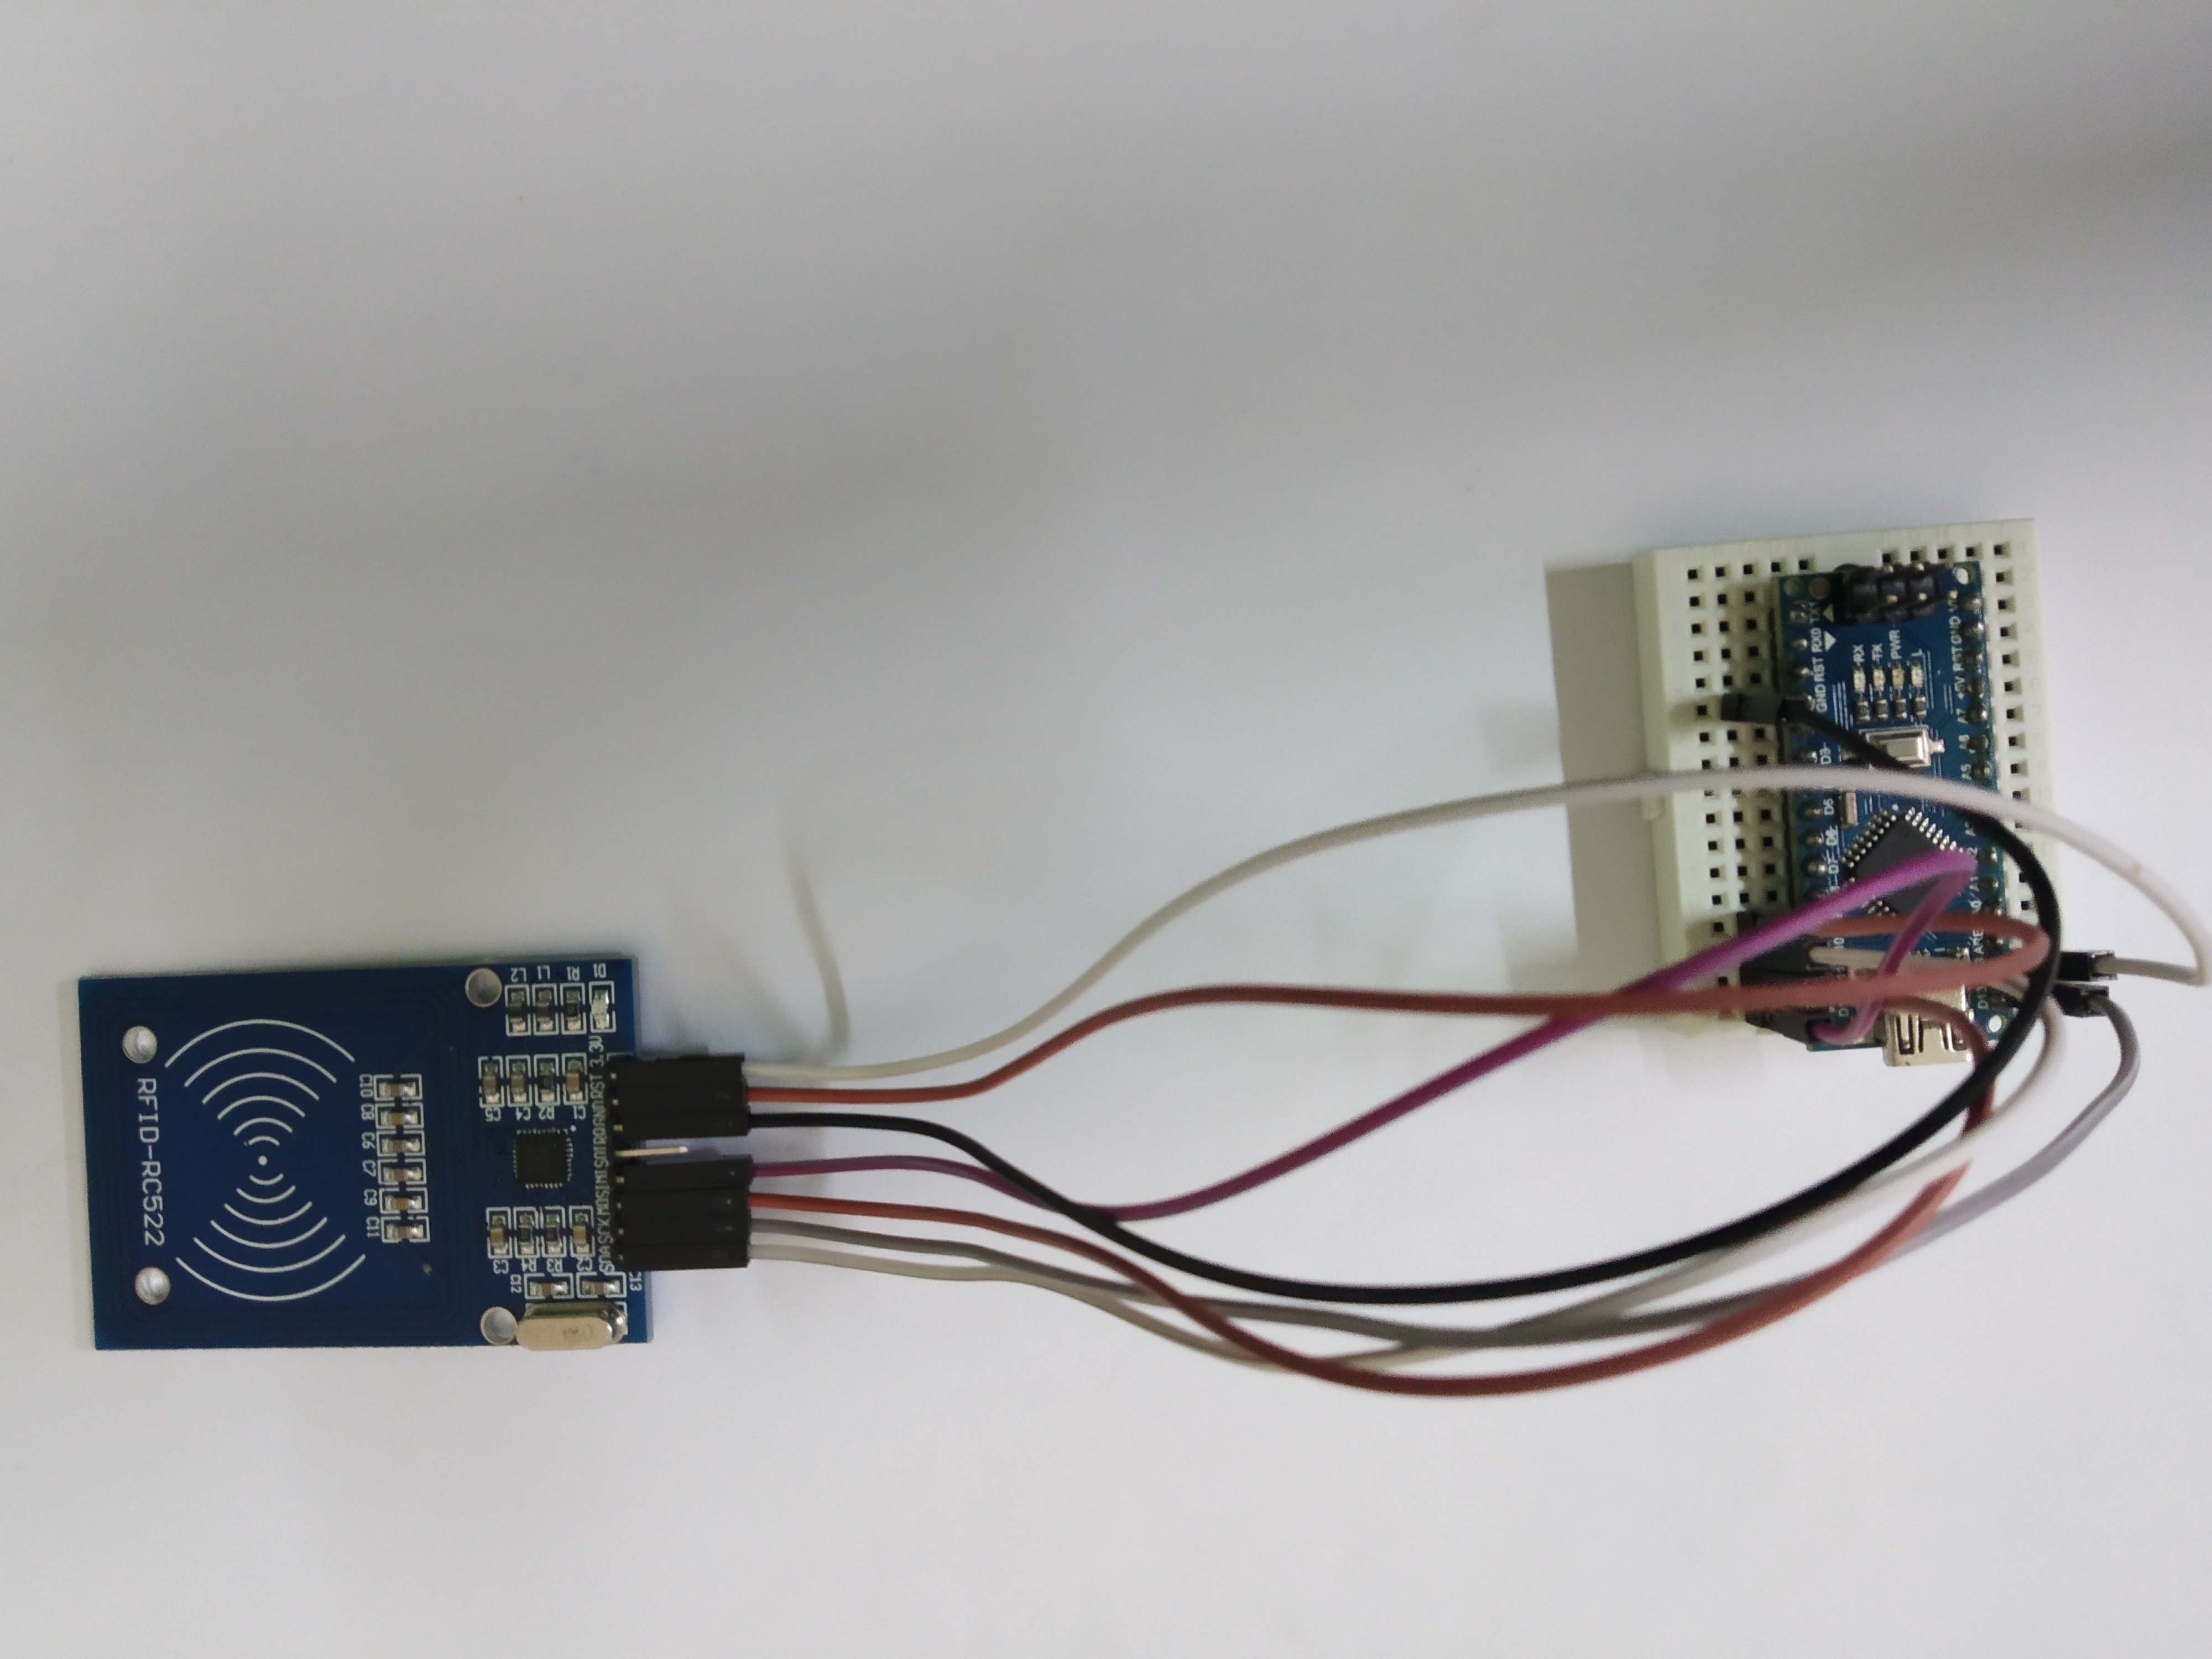
\includegraphics[width=0.7\textwidth]{Figuras/prototype_arduino.png}            \legend{Fonte: Própria}
\end{figure}\begin{figure}[H]
              \caption{\label{fig:prototipo_nodemcu}{Protótipo NodeMcu}}
              \centering
              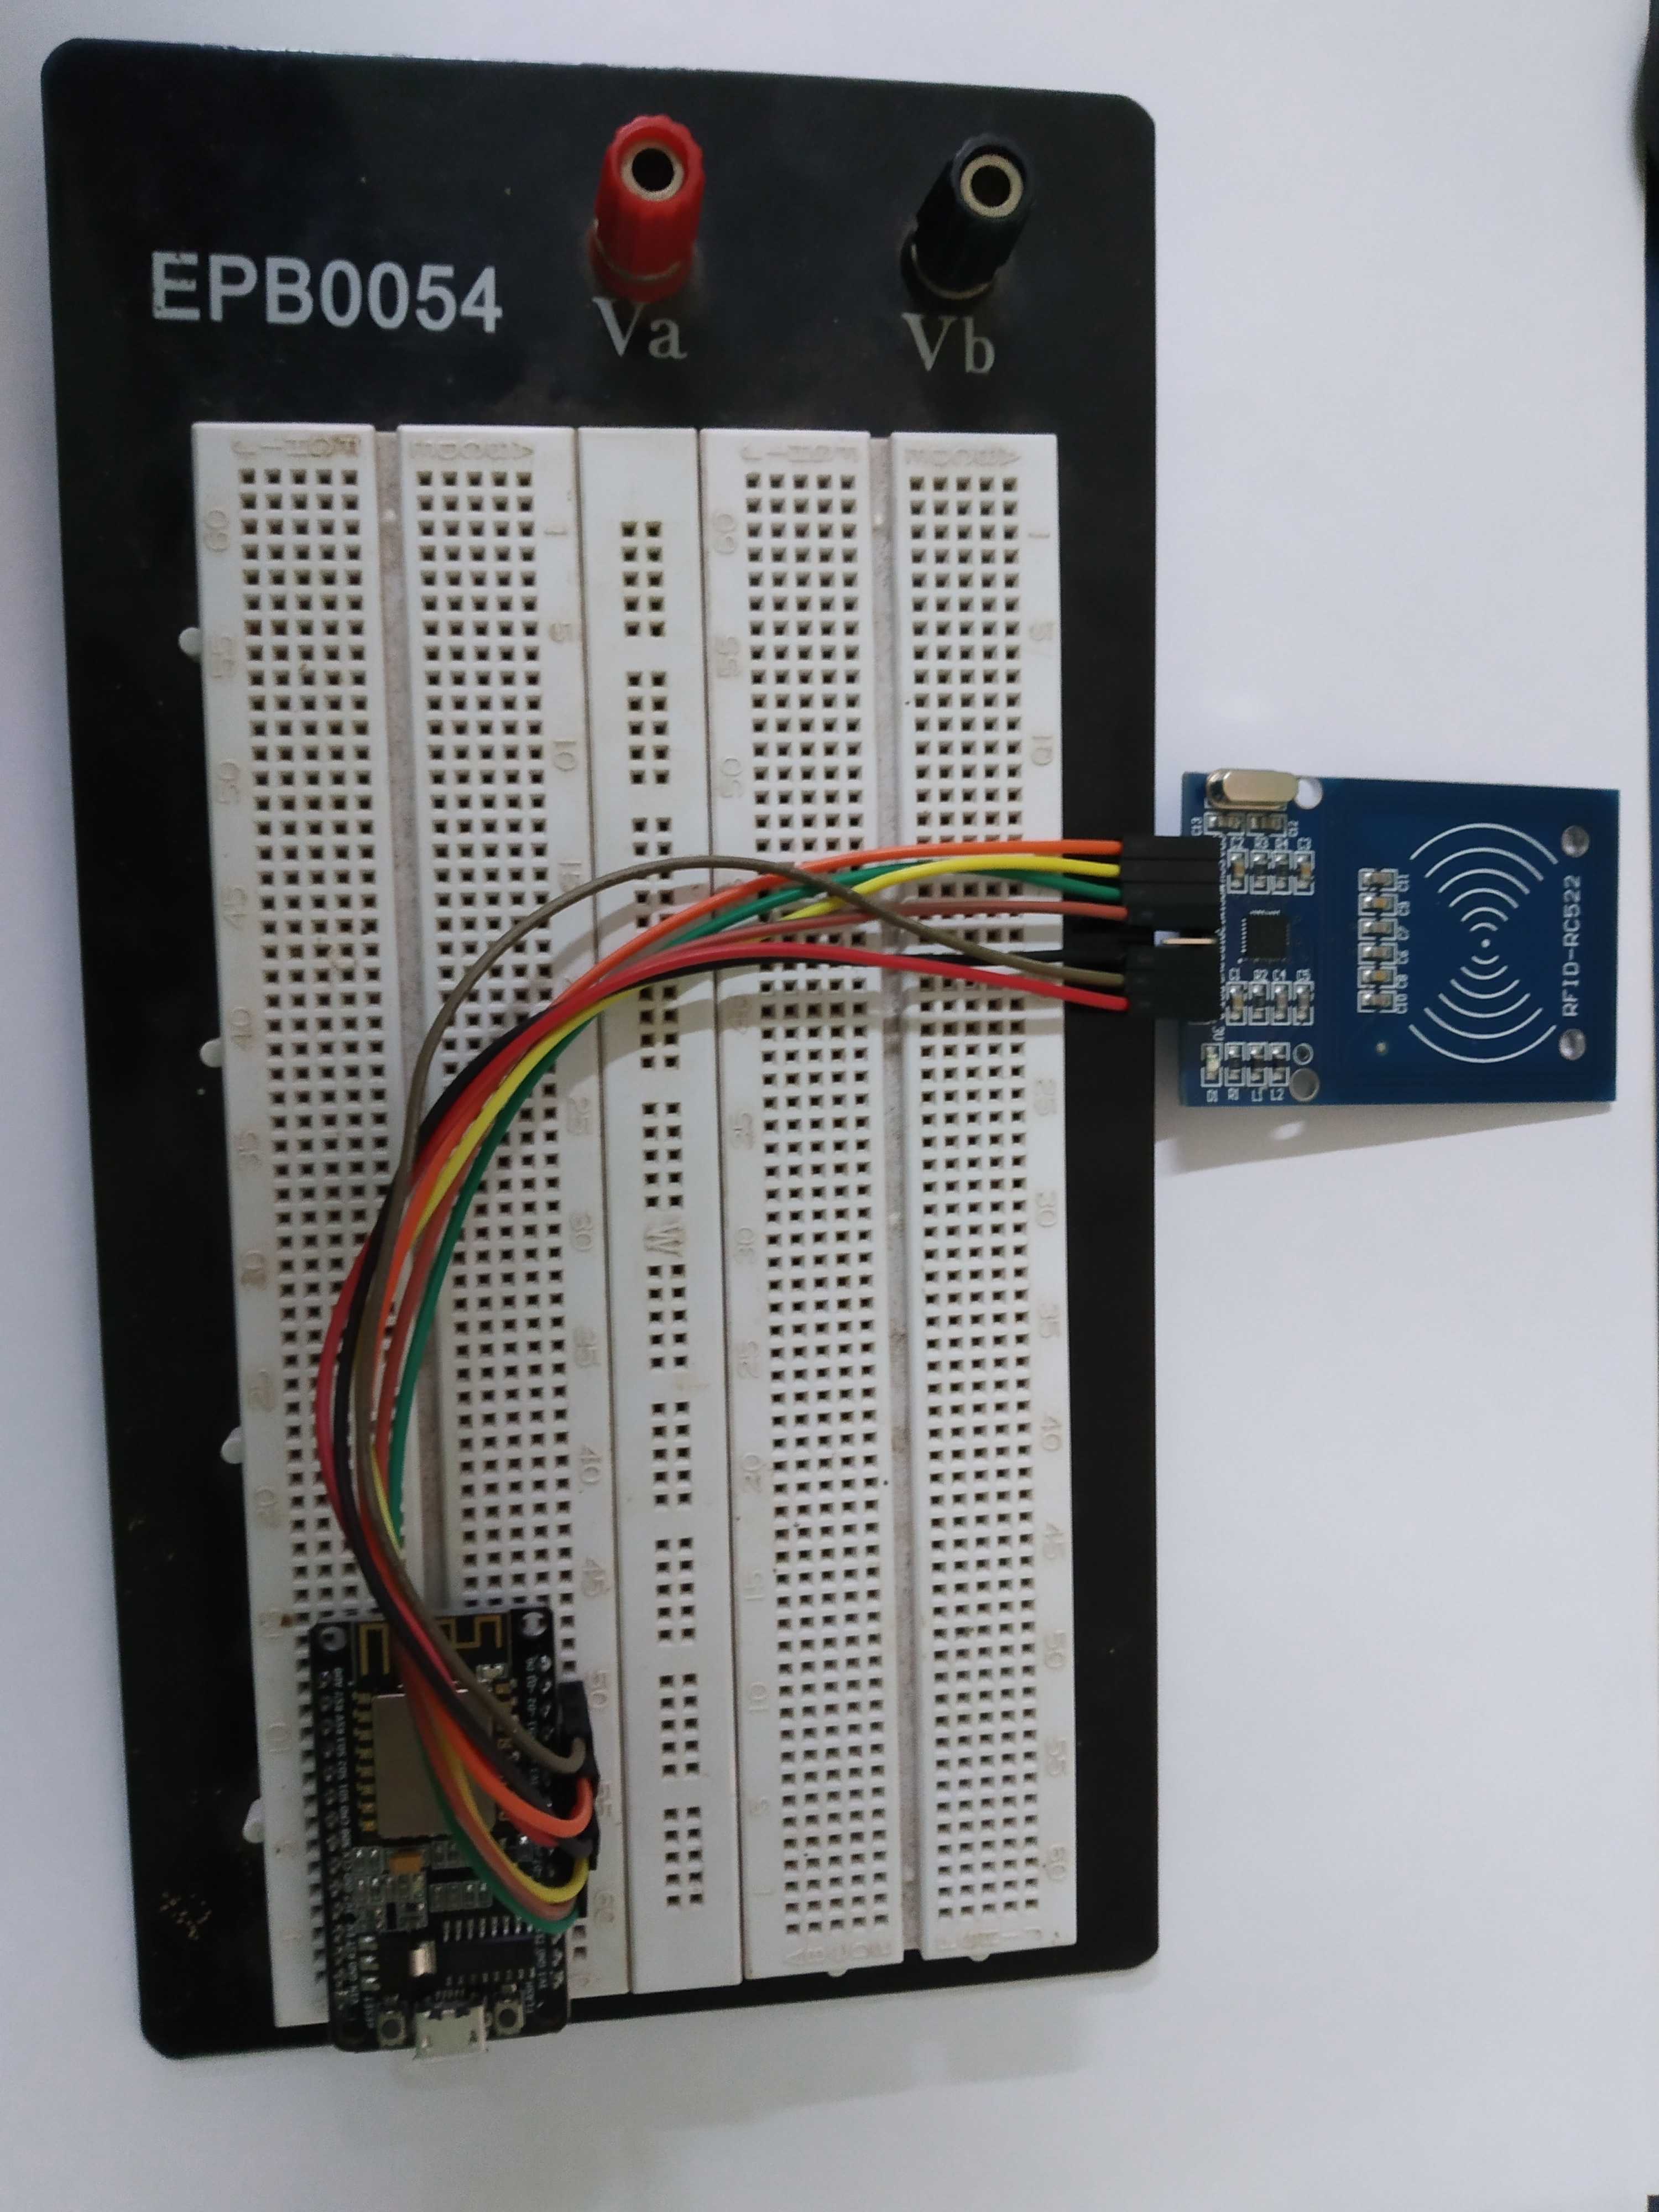
\includegraphics[width=0.5\textwidth]{Figuras/prototype_nodemcu.png}
              \legend{Fonte: Própria}
\end{figure}


\par
Para a simulação do servidor, foi utilizado um notebook com $6GB$ de memória RAM, processador Intel Core $i5-4200$, HD de $750GB$, placa de video GeForce $720M$ de $2GB$ de memória dedicada e sistema operacional Windows $10$ Home Single Language. A rede LAN utilizada foi criada através de um roteador \textit{TP-LINK} modelo $TL-WR720N$. Também foram utilizadas quatro etiquetas RFID passivas, cada uma dessas etiquetas representa um objeto diferente para a simulação.

\todo[color=green,inline]{Sugiro descrever cada um dos cenários propostos na avaliação para responder as questões de pesquisa.}
\par
A execução do experimento aconteceu no cenário apresentado na \autoref{fig:cenario}, foi simulado duas salas e quatro objetos rastreáveis em um edifício. Visando responder as questões foram executados os seguintes testes: (1) localização e identificação dos objetos, no intuído de obter respostas para a primeira pergunta, (2) criação de restrição de objeto afim de verificar se as notificações ao violar restrição são uma forma de se ter melhor gerenciamento dos objetos e (3) levantamento de todos os objetos e as salas que eles estão \todo[color=green]{Mover este texto para seção anterior, e ampliar a descrição focando as questões de pesquisa}.

\begin{figure}[H]
              \caption{\label{fig:cenario}{Cenário de simulação}}
              \centering
              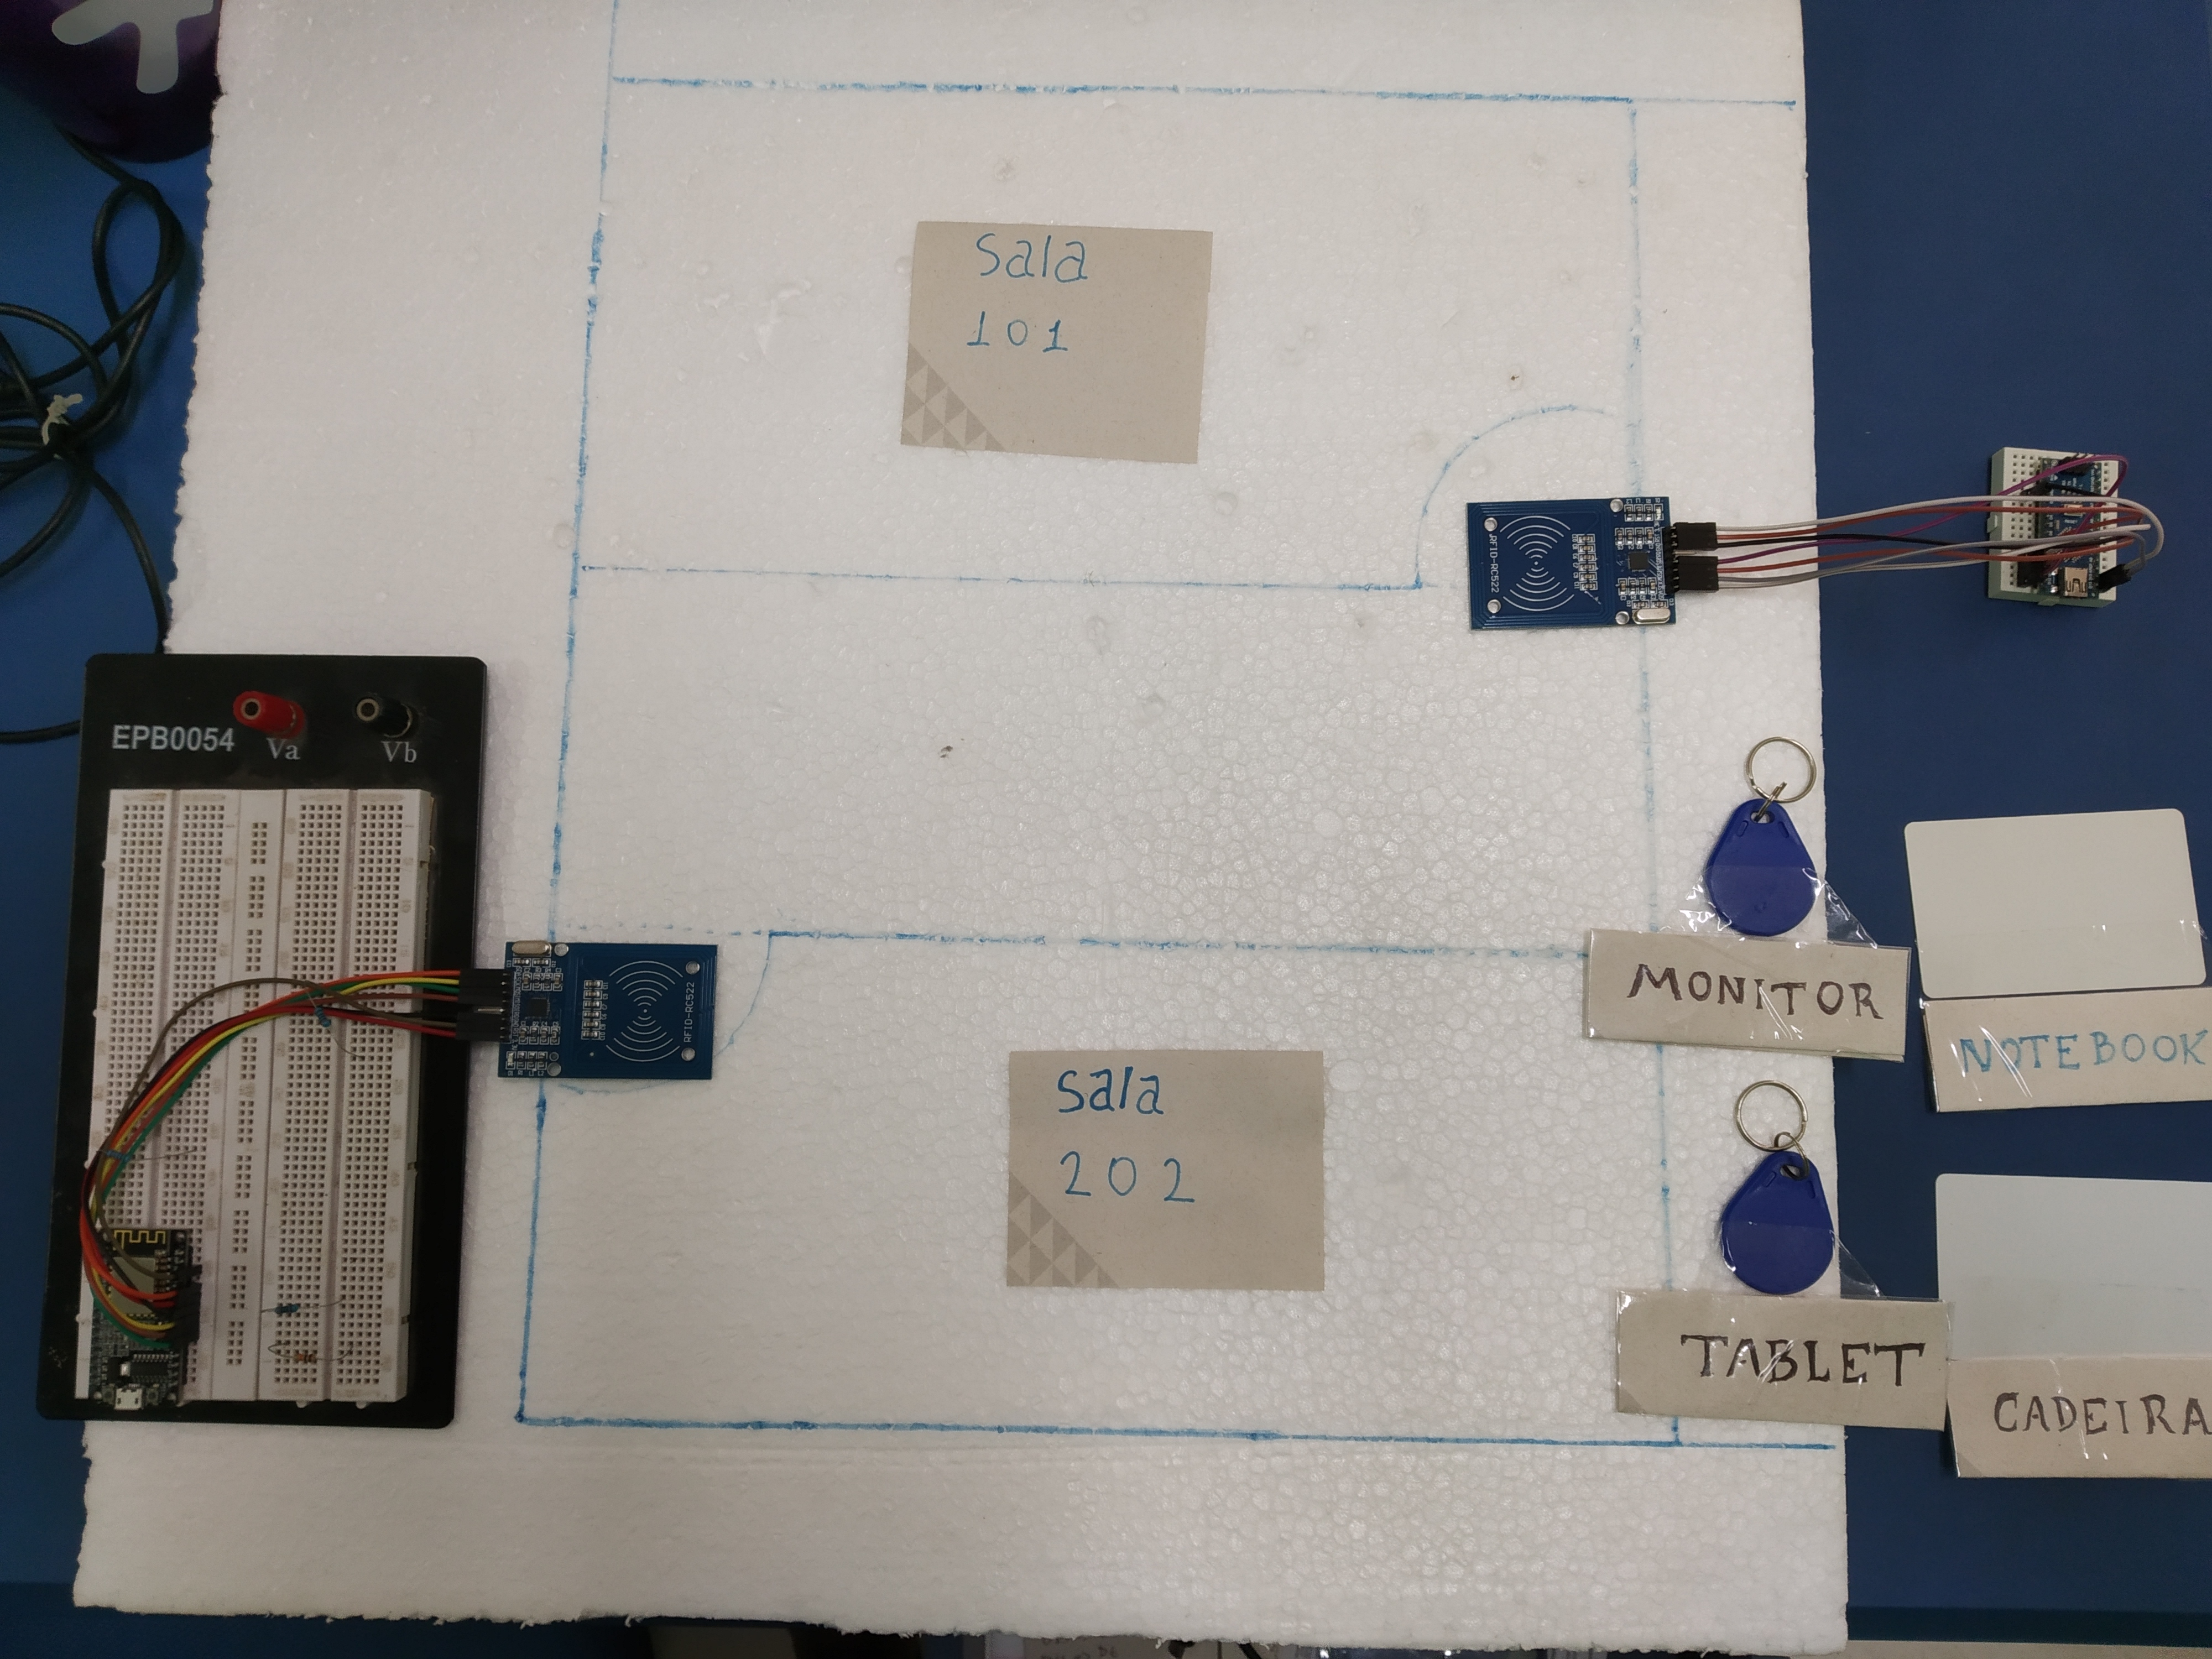
\includegraphics[width=1\textwidth]{Figuras/cenario.png}
              \legend{Fonte: Própria}
\end{figure}
\section{Execução dos experimentos e Análise dos Resultados}

\todo[inline]{A partir daqui você deve descrever os resultados de forma detalhada e respondendo as questões de pesquisa}
 
 Visando responder as questões do planejamento, iniciamos os testes do cenário (1) cadastrando as quatro etiquetas no sistema e identificando-as cada uma como um objeto diferente, duas etiquetas foram lidas pelo dispositivo de porta da sala $101$ e as outras duas foram lidas pelo dispositivo de porta da sala $202$, o \textit{pipiline} do processo pode ser visualizado na \autoref{fig:piptransicao} de A até D, esse processo foi repetido mais três vezes e o resultado final desse processo com as quatro etiquetas esta na ultima figura.

\begin{figure}[ht]
        \centering\caption{Identificação dos objeto}
        \label{fig:piptransicao}
       \subfloat[A\label{fig:execution1a}]{
            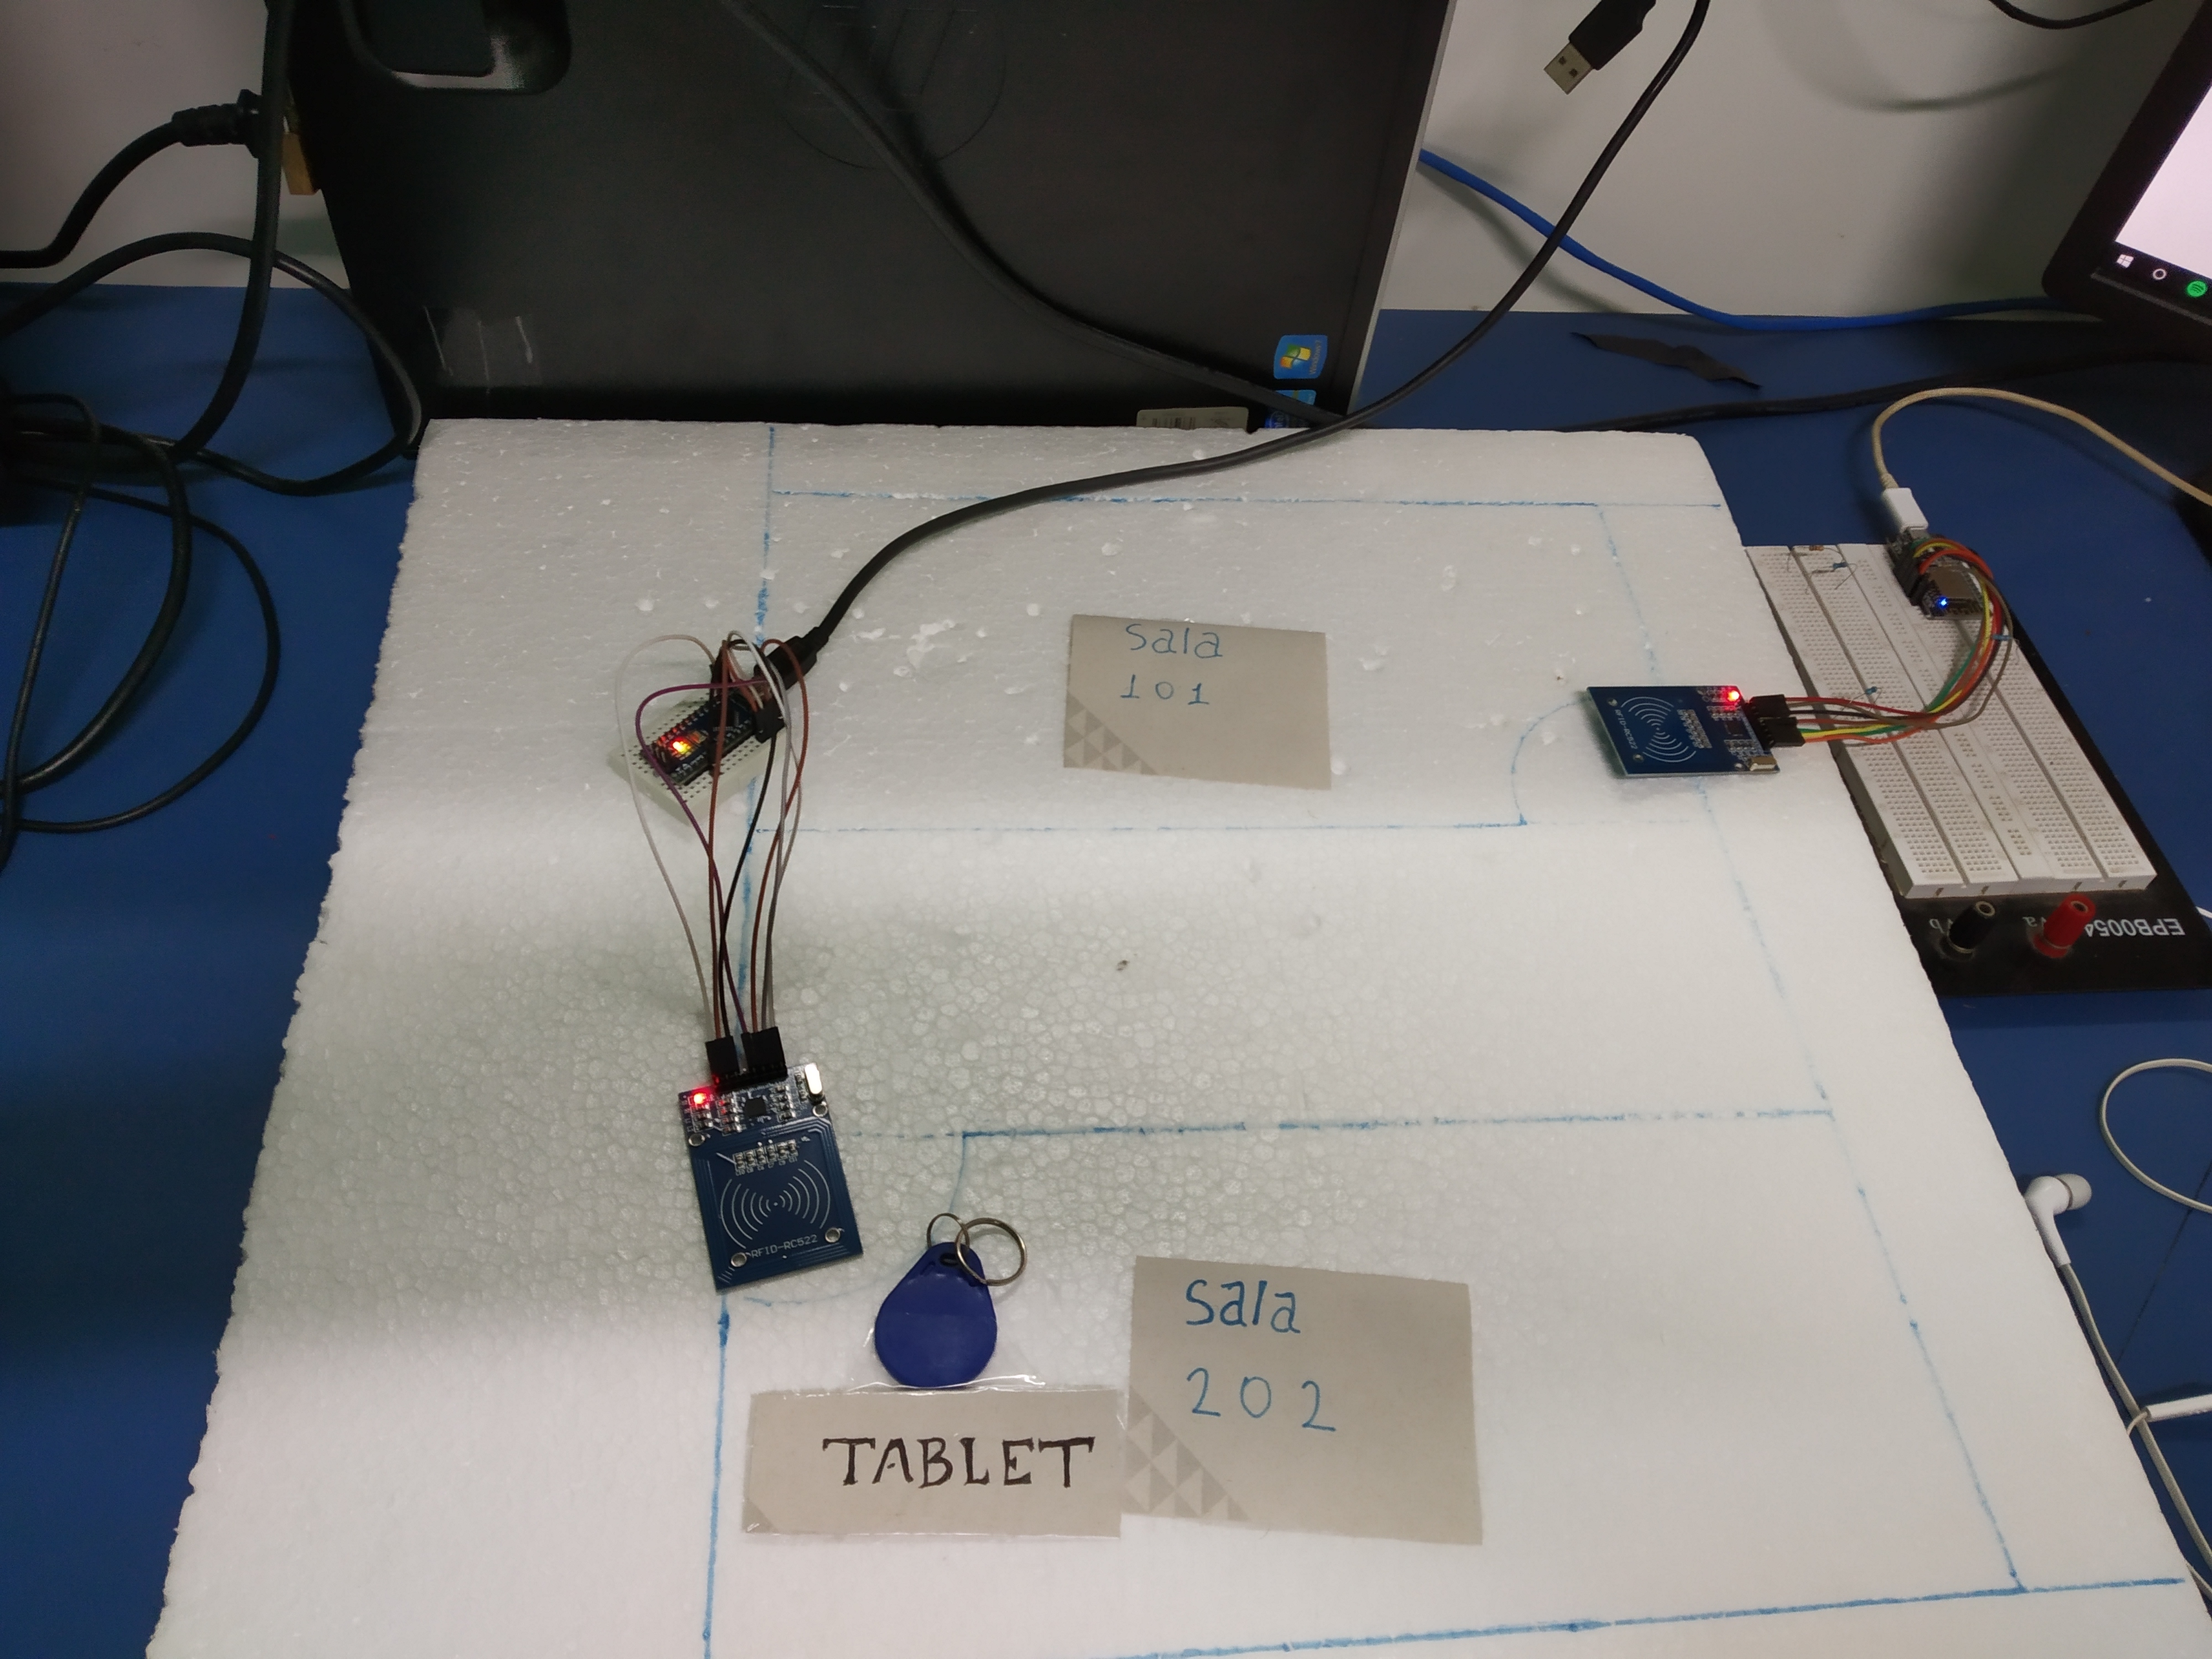
\includegraphics[width=0.4\textwidth]{Figuras/execucao1a.PNG}}
         \hspace{0.5cm}
       \subfloat[B\label{fig:execution1b}]{
            \includegraphics[width=0.4\textwidth]{Figuras/execucao1.PNG}}
             \hspace{0.5cm}
       \subfloat[C\label{fig:execution1c}]{
            \includegraphics[width=0.4\textwidth]{Figuras/execucao1br.PNG}}
        \hspace{0.5cm}
       \subfloat[D\label{fig:execution1d}]{
            \includegraphics[width=0.4\textwidth]{Figuras/execucao1c.PNG}}
             \hspace{0.5cm}
       \subfloat[E\label{fig:execution1f}]{
             \includegraphics[width=0.4\textwidth]{Figuras/execution1F.PNG}}
              \hspace{0.5cm}
      \legend{Fonte: Própria}
\end{figure}

\par
Ainda realizando teste no cenário (1), executamos o processo de transição dos objetos onde uma etiqueta é lida quando sai da sala e quando entra na outra sala, esse \textit{pipiline} pode ser visto na \autoref{fig:piptransicao} de \texttt{A} até \texttt{E}. Foram executadas transições para todos objetos onde os objetos que estavam na sala 101 ficaram na sala 202 e os da sala 202 foram para a sala 101.

\begin{figure}[ht]
        \centering\caption{Transição de objeto}
        \label{fig:piptransicao}
       \subfloat[A\label{fig:execution2a}]{
            \includegraphics[width=0.4\textwidth]{Figuras/execution2a.png}}
         \hspace{0.5cm}
       \subfloat[B\label{fig:execution2b}]{
            \includegraphics[width=0.4\textwidth]{Figuras/execution2c.png}}
             \hspace{0.5cm}
       \subfloat[C\label{fig:execution2c}]{
            \includegraphics[width=0.4\textwidth]{Figuras/execution2b.png}}
        \hspace{0.5cm}
       \subfloat[D\label{fig:execution2d}]{
            \includegraphics[width=0.4\textwidth]{Figuras/execution2d.png}}
             \hspace{0.5cm}
       \subfloat[E\label{fig:execution2c}]{
             \includegraphics[width=0.4\textwidth]{Figuras/execution2e.png}}
              \hspace{0.5cm}
        
      \legend{Fonte: Própria}
\end{figure}

\par
No cenário (2), foram criados dois usuário na tela de quem notificar para receber as notificações via email, para isso foi utilizado o email's do próprio autor, em seguida foi criado restrição para cada objeto. Na tela principal cada objeto possui uma opção para editar ao seu lado, foi editado um objeto por vez colocando no campo restrição o mesmo nome que ele possuía no campo de \texttt{localização(sala)}. O cadastro dos usuários e a edição dos objetos pode ser visualizado no \textit{pipiline} da \autoref{fig:cadRest}.

\begin{figure}[ht]
        \centering\caption{Cadastro de usuários e Criação de Restrições de objeto}
        \label{fig:cadRest}
       \subfloat[A\label{fig:execution3a}]{
            \includegraphics[width=0.4\textwidth]{Figuras/execution3a.png}}
         \hspace{0.5cm}
       \subfloat[B\label{fig:execution3b}]{
            \includegraphics[width=0.4\textwidth]{Figuras/execution3b.png}}
             \hspace{0.5cm}
       \subfloat[C\label{fig:execution3c}]{
            \includegraphics[width=0.4\textwidth]{Figuras/execution3c.png}}
        \hspace{0.5cm}
       \subfloat[D\label{fig:execution3d}]{
            \includegraphics[width=0.4\textwidth]{Figuras/execution3d.png}}
             \hspace{0.5cm}
       \subfloat[E\label{fig:execution3e}]{
             \includegraphics[width=0.4\textwidth]{Figuras/execution3e.png}}
              \hspace{0.5cm}
      \legend{Fonte: Própria}
\end{figure}
\par
Ainda no cenário (2), foi realizado processo de transição com os objetos afim de verificar se o sistema notifica os usuários através do e-mail e na tela inicial, o \textit{pipiline} da execução esta na \autoref{fig:transicaoeRest}. Foram realizadas transições para todos os objetos com restrições.

\begin{figure}[ht]
        \centering\caption{Transições com Restrições}
        \label{fig:transicaoeRest}
       \subfloat[A\label{fig:execution4a}]{
            \includegraphics[width=0.4\textwidth]{Figuras/execution4a.png}}
         \hspace{0.5cm}
       \subfloat[B\label{fig:execution4b}]{
            \includegraphics[width=0.4\textwidth]{Figuras/execution4b.png}}
             \hspace{0.5cm}
       \subfloat[C\label{fig:execution4c}]{
            \includegraphics[width=0.4\textwidth]{Figuras/execution4c.png}}
        \hspace{0.5cm}
       \subfloat[D\label{fig:execution4d}]{
            \includegraphics[width=0.4\textwidth]{Figuras/execution4d.png}}
             \hspace{0.5cm}
       \subfloat[E\label{fig:execution4c}]{
             \includegraphics[width=0.4\textwidth]{Figuras/execution4e.png}}
              \hspace{0.5cm}
        \subfloat[E\label{fig:execution4d}]{
             \includegraphics[width=0.4\textwidth]{Figuras/execution4e.png}}
              \hspace{0.5cm}      
        \subfloat[E\label{fig:execution4e}]{
             \includegraphics[width=0.4\textwidth]{Figuras/execution4e.png}}
              \hspace{0.5cm}
      \legend{Fonte: Própria}
\end{figure}
No cenário (3) é o levantamento de todos objetos cadastrados no sistema com suas respectivas salas, primeiramente é necessário ir até a tela \texttt{Ger. de Salas} para verificar as salas cadastradas no sistema e em seguida ir para a tela \texttt{Inventário}. O \textit{pipiline} das duas execuções desse processo está na \autoref{fig:invent}.

\begin{figure}[ht]
        \centering\caption{Inventário}
        \label{fig:invent}
       \subfloat[A\label{fig:execution5a}]{
            \includegraphics[width=0.4\textwidth]{Figuras/execution5a.png}}
         \hspace{0.5cm}
       \subfloat[B\label{fig:execution5b}]{
            \includegraphics[width=0.4\textwidth]{Figuras/execution5b.png}}
             \hspace{0.5cm}
       \subfloat[C\label{fig:execution5c}]{
            \includegraphics[width=0.4\textwidth]{Figuras/execution5c.png}}
        \hspace{0.5cm}
       \subfloat[D\label{fig:execution5d}]{
            \includegraphics[width=0.4\textwidth]{Figuras/execution5d.png}}
             \hspace{0.5cm}
       \subfloat[E\label{fig:execution5c}]{
             \includegraphics[width=0.4\textwidth]{Figuras/execution5e.png}}
              \hspace{0.5cm}
        
      \legend{Fonte: Própria}
\end{figure}
\subsection{Resultados}

Após a execução dos testes, foram obtidos os resultados apresentados na \autoref{tab:resultados}, onde cada linha representa um cenário de execução com os números de execuções, número de execuções que funcionaram, números de execuções que funcionaram mas por alguma questão não funcionou perfeitamente, e as que falharam.

\todo[inline, color=green]{Adicionar figuras com a execução de cada cenário, discutindo as ações em termos de vantagens e desvantagens da execução do sistema}
\todo[inline]{Seria bom relacionar a execução dos cenários as tecnologias usadas no sistema}
\begin{table}[htbp]
  \caption{Resultados}
  \label{tab:resultados}
  \begin{tabularx}{\textwidth}{|X|c|c|c|c|c|}
     \hline
    & \textbf{N$^{\circ}$ de execuções} & \textbf{Funcionou } & \textbf{Parcialmente} & \textbf{Falhou} \\
    \hline
    Cenário 1 & 4 & 3 & & 1\\
    \hline
    Cenário 2 & 4 & 4 &  &\\
    \hline
     Cenário 3 & 2 & 1 & 1 &\\
    \hline

  \end{tabularx}
\end{table}

\par
O INEXT conseguiu localizar objetos em ambientes confinados, porém o sistema não proporciona a posição real do objeto no ambiente, o sistema também foi capaz de identificar os objetos mas essa etapa ainda ocorre de maneira manual necessitando ser realizada por usuários. Durante os teste houve uma execução em que os \textit{script} em Python travou e não enviou o JSON gerado para o servidor e ocasionando a perda da localização de um objeto, essa é a execução cujo esta na tabela que falhou.

\par
O sistema proporcionou uma boa forma de gerenciar os objetos de forma que conseguiu informar os usuários sobre as violação de restrições através do e-mail e também da tela principal do sistema, gerando uma nova tabela com os objetos que violaram suas restrições.

\par
Durante a primeira tentativa de gerar o inventário dos objetos cadastrados no sistema, houve repetição de dados justamente porque foram criadas salas repetidas no banco de dados, para solucionara esse problema foi necessário ir até a tela \texttt{Ger. de Salas} e remover as salas repetidas, dessa forma a geração do inventário funcionou sem a repetição dos objetos e salas.

\par


%\chapter{DISCUSSÃO}

% ----------------------------------------------------------
% Conclusão
% ----------------------------------------------------------
\chapter{CONSIDERAÇÕES FINAIS E TRABALHOS FUTUROS}

\label{chapter:consideracoes}

Este trabalho propôs um sistema de localização e identificação de objetos em edifícios por meio de
radiofrequência, usando etiquetas passivas. O real objetivo consiste em facilitar e auxiliar o gerenciamento/controle de
bens em edifícios cujo possuem uma grande quantidade de salas.

%\todo[inline]{Adicionar um text resumido sobre os resultados dos experimentos}

\par
O método até o momento possui limitações referente ao leitor RFID utilizado, o leitor possui o alcance baixo necessitando que as etiquetas sejam praticamente encostadas para que a leitura seja realizada, sendo necessário a substituição do leitor caso o sistema seja implantado em um prédio.
\par
Os experimentos realizados demonstraram que o sistema ainda precisa de melhorias para que se torne um produto final, por outro lado a proposta tem pontos positivos e satisfatórios. Um dos pontos a ser melhorado é a necessidade de ter que remover as salas repetidas antes de gerar o inventário, outra melhoria seria a possibilidade de gerar o inventário de apenas uma sala por vez.

\par
O questionário com pessoas que já foram ou ainda possuem cargo de chefia ou coordenador de departamentos de cursos na universidade indicaram que o sistema pode proporcionar mais facilidade nas tarefas de gerenciamento ou servir como ferramenta de auxilio, de forma que mostra a viabiliadade do sistema como resultado do questionário.
\par

%Neste trabalho já foram obtidos alguns resultados parciais em relação a identificação de componentes de hardware como o módulo wireless ESP-8266 e o Módulo Leitor Rfid Mfrc522 Mifare, bem como, alguns testes iniciais que apontam a viabilidade para a construção de um protótipo. Desta forma, os próximos passos deste trabalho visam o desenvolvimento e testes do sistema proposto para análise da localização dos objetos. 
Adicionalmente, visa-se estudar métodos para ter uma localização mais precisa sobre a localização dos objetos, por exemplo, pode-se utilizar etiquetas ativas para auxiliar e em seguida aplicar algoritmos de RSSI, dessa forma tende-se a ter uma localização com maior precisão no ambiente e uma maneira para executar o processo de identificação dos objetos de maneira automática. 




%\newpage
% ----------------------------------------------------------
\chapter{ANEXO A}
% \label{chapter:anexo}
\section{Lista de imagens das telas}
\begin{figure}[H]
              \caption{\label{fig:tela_inical2}Tela Inicial }
              \centering
              \includegraphics[width=0.9\textwidth]{Figuras/tela_inical2.PNG}
              \legend{Fonte: Própria}
    \end{figure}
    
    \begin{figure}[H]
              \caption{\label{fig:tela_cadastro_manual}Tela de Cadastro de Objeto Manual}
              \centering
              \includegraphics[width=0.9\textwidth]{Figuras/tela_cadastro_manual.png}
              \legend{Fonte: Própria}
    \end{figure}
    
    \begin{figure}[H]
              \caption{\label{fig:tela_cadastro_manual}Tela de Editar Objeto}
              \centering
              \includegraphics[width=0.9\textwidth]{Figuras/tela_editar.png}
              \legend{Fonte: Própria}
    \end{figure}
    
     \begin{figure}[H]
              \caption{\label{fig:tela_cadastro_manual}Tela de Quem Notificar}
              \centering
              \includegraphics[width=0.9\textwidth]{Figuras/tela_quem_notificar.PNG}
              \legend{Fonte: Própria}
    \end{figure}
    
    \begin{figure}[H]
              \caption{\label{fig:tela_cadastro_manual}Tela de Editar ADM}
              \centering
              \includegraphics[width=0.9\textwidth]{Figuras/tela_editar_adm.png}
              \legend{Fonte: Própria}
    \end{figure}
    
    \begin{figure}[H]
              \caption{\label{fig:tela_inventario}Tela de Inventário}
              \centering
              \includegraphics[width=0.9\textwidth]{Figuras/tela_inventario.png}
              \legend{Fonte: Própria}
    \end{figure}
    
    \begin{figure}[H]
              \caption{\label{fig:tela_ger_sala}Tela de Ger. Sala}
              \centering
              \includegraphics[width=0.9\textwidth]{Figuras/tela_ger_sala.png}
              \legend{Fonte: Própria}
    \end{figure}
%\newpage
% ----------------------------------------------------------
% ----------------------------------------------------------
% \chapter{APÊNDICE A}
\section{Revisão Sistemática}

Nesta seção é apresentado o protocolo definido para a aplicação e execução da revisão sistemática que foi parcialmente executada
neste trabalho, devido ao tempo e quantidade de publicações\todo{Adicionar o número de artigos da execução da string de busca} 
identificadas. Todos os artigos citados na Seção~\ref{chapter:correlatos} foram selecionados através da execução deste protocolo proposto.
%execução de uma revisão sistemática da literatura, parcialmente executada, conforme descrito  detalhadamente no \autoref{chapter:apendice1} - Apêndice $1$.

			Segundo \citeauthor{Kitchenham:2009:SLR:1465742.1466091}  a revisão sistemática é uma seleção da literatura que segue um protocolo formal, sendo uma revisão metodologicamente rigorosa dos resultados e com o objetivo de agregar todas as evidências existentes em uma pesquisa. A sua aplicação consiste em umas sequência de passos definidos a ser seguidos e se comparado a revisão da literatura informal requer um grande esforço.
			
			\par 
			A revisão sistemática atua como um meio de identificação  e avaliação para pesquisa conduzindo-o para tópicos relevantes sobre o tema de interesse, diferentemente da revisãos da literatura informal em que a presença de variações entre os estudos representa um fator negativo
			\cite{MafraTravassos}. 
			De acordo com \citeauthor{MafraTravassos} o processo da revisão sistemática envolve três etapa: 
			\begin{enumerate}
			    \item \textbf{Planejamento da Revisão}: nesta etapa os objetivos são listado e é definido o protocolo de revisão;
			    \item \textbf{Condução da Revisão}: etapa onde as fontes para a revisão sistemática são selecionados, identificação de estudos primários e avaliados com critérios de inclusão e exclusão;
			    \item \textbf{Publicação dos Resultado}: na terceira etapa os dados dos estudos são extraídos e sintetizados para serem publicados.
			\end{enumerate}
			
			\par 
			Conduzimos a revisão deste trabalho com a finalidade de realizar um estudo exploratório de caracterização da área, e assim podemos afirmar que essa revisão se caracteriza como uma quasi-sistemática pois está baseada nas três etapas citada anteriormente \cite{MafraTravassos}, seguindo o processo da revisão sistemática e preservando o rigor e o mesmo formalismo para as fases metodológicas de elaboração e execução do protocolo, faltando apenas uma meta-análise do que poderia ser aplicado futuramente.
			

		\subsection{ Planejamento da Revisão Sistemática}
			\par
\textbf{Objetivo: }O objetivo desta revisão é analisar publicações científicas com o propósito de  identificar métodos para a localização de objetos com a utilização de tag RFID no contexto acadêmico ou industrial.
			
            \par
            \textbf{Formulação das Perguntas.}
            
            \begin{itemize}
              \item Quais os métodos para a localização de tags RFID?
              \item Está disponível alguma ferramenta para localização de tags RFID ?
              \item Quais as limitações em relação a identificação de mais de uma tag RFID simultaneamente?
              \item Quais os requisitos necessários para execução do método?
              \item Quais as limitações do método proposto ?
              \item Quais são as perspectivas futura para a melhoria do método e da aplicação?

            \end{itemize}
			
            \begin{itemize}
            \item \textbf{População}
            	\begin{itemize}
            		\item \textbf{Palavras-Chave} "tag RFID"  OR  "RFID signaling scheme"  OR  "RFID reader"  OR  "Handheld RFID Reader"  OR  "RFID Label"  OR  "RFID Tag Reader"  OR  "Passive RFID Tags"  OR  "Passive RFID Readers" OR “Radio-Frequency IDentification” OR “Radio Frequency IDentification”  OR “review of RFID” OR “RFID  technology” OR “RFID localization” OR “method for RFID” OR “Active RFID”
            	\end{itemize}
            \item \textbf{Intervenção } 
            	\begin{itemize}
            
             \item \textbf{Palavras-Chave} “Positioning principles” OR "object localization indoor"  OR  "positioning algorithms"  OR  "indoor location technique"  OR  "indoor object management"  OR  "asset localization"  OR  "localization-based services"  OR  "facilities management"  OR  "pattern matching"  OR  "mapping"  OR  "indoor automatic identification"  OR  "indoor tag classification"  OR  "indoor classify RFID"  OR  "indoor classify tag"  OR  "indoor localization techniques" OR “Applications and techniques” OR “system for indoor” OR “real-time locating” OR “localization method” OR “tags for indoor” OR “Efficient object localization” OR “using RSS” OR “algorithms and applications” AND NOT “using UHF RFID”
           		\end{itemize}
            \end{itemize}
             
            
	\subsection{Procedimento de Seleção de Critérios}

	  		\begin{itemize}
      			\item \textbf{CE1-01}: Não serão selecionadas publicações em que não contém as  palavras-chave da string de busca no título, resumo, método  e/ou resultados. Os campos de seções de agradecimentos, biografia dos autores, referências bibliográficas e anexos não serão incluídos.

      			\item \textbf{CE1-02}: Publicações cujo se assemelham com  tutoriais e cursos não serão selecionadas.

      			\item \textbf{CE1-03}: Não serão selecionadas publicações em que técnicas e algoritmos  para localização de objetos não trabalham com identificação por rádio frequência (RFID).

      			\item \textbf{CE1-04}: Não serão selecionadas publicações em que façam utilização de frequência ultra-alta (UHF) RFID.

      			\item \textbf{CE1-05}:  Não serão selecionadas publicações que não fazem uma abordagem para utilização de RFID para localizar objetos com tags RFID.
    	\end{itemize}
	\par
	Publicações que podem ser incluídas no conjunto.

	\begin{itemize}
    	\item \textbf{CI1-01}: Podem ser selecionadas publicações em que o contexto das palavras-chave utilizadas no artigo leva a crer que faz uma citação para uma abordagem de utilização de RFID para localizar objetos utilizando tags RFID.
        \item \textbf{CI1-02} Podem ser selecionadas publicações em que o contexto das palavras-chave utilizadas no artigo leva a crer que a publicação cita recomendações de algoritmos, métodos e ferramentas que possam ser utilizados para localizar objetos com tag RFID.
    \end{itemize}

%\newpage
% ----------------------------------------------------------
% Referências bibliográficas
% ----------------------------------------------------------
\addto\captionsportuguese{\renewcommand{\bibname}{Referências}}
\renewcommand{\bibname}{Referências}
\bibliography{main}

%---------------------------------------------------------------------
% INDICE REMISSIVO
%---------------------------------------------------------------------
%\phantompart
%\printindex
%---------------------------------------------------------------------

\end{document}

